\documentclass[11pt,a4paper]{article}
\PassOptionsToPackage{obeyspaces}{url}
\usepackage[margin=2.3cm]{geometry}
\usepackage{amsmath,amssymb,bm}
\usepackage{graphicx}
\usepackage{booktabs,longtable,array}
\usepackage[table]{xcolor}
\usepackage{microtype}
\usepackage[numbers,sort&compress]{natbib}
\usepackage[colorlinks=true,linkcolor=blue!50!black,citecolor=green!40!black,urlcolor=blue!60!black]{hyperref}
\usepackage{url}
\numberwithin{equation}{section}
\graphicspath{{figs/}}
\newcommand{\sq}{\sqrt{f_R}}
\newcommand{\dd}{\mathrm{d}}
\newcommand{\jh}{\hat\jmath_\ell}
\newcommand{\yh}{\hat y_\ell}
\newcommand{\RR}{\mathcal R}
\newcommand{\TT}{\mathcal T}
\newenvironment{verifbox}{\par\medskip\begingroup\small\noindent{\color{orange!70!black}\rule{\linewidth}{0.8pt}}\par\nopagebreak\noindent\textbf{\color{orange!70!black}Second-round verification.}\ }%
  {\par\nopagebreak\noindent{\color{orange!70!black}\rule{\linewidth}{0.8pt}}\par\endgroup\medskip}
\sloppy

\title{Gravitational waves and a spherical thin shell:\\[2pt]
\large linearized junction conditions, scattering coefficients, quasinormal modes\\
and the dynamical fate of the background}
\author{A complete account of the first-round work (``First round'' folder),\\
written and verified in the second round}
\date{25 September 2026}

\begin{document}
\maketitle

\begin{abstract}
We give a self-contained account of a computation of gravitational-wave scattering off, and of the
quasinormal modes (QNMs) of, a spherical thin shell that separates a flat interior from a Schwarzschild exterior.
Both parities are treated: odd (Regge--Wheeler, Cunningham--Price--Moncrief) and even (Zerilli--Moncrief).
The first obstacle is physical. A pure domain wall, the object of the prior notes, has no static configuration:
it always collapses. We examine every way out. A static dust shell does not exist. A static perfect-fluid
shell exists, but its pressure-to-density ratio is fixed by the compactness (model C). A domain wall can be frozen at its
turning point (model A). The linearized Israel junction conditions are then derived from first principles and
verified symbolically. In the odd sector they reduce, for every perfect-fluid shell, to continuity of the master
function and a repulsive $\delta$-function potential of strength $\Delta_{\rm odd}=\sq(1-\sq)/R$ in the tortoise
coordinate. In the even sector they form a frequency-dependent $2\times2$ transfer matrix that encodes the radial
displacement of the shell in the two Regge--Wheeler gauges and the motion of its matter. Reflection and transmission
coefficients are defined by opening the interior, and satisfy $\RR+\TT=1$ to $10^{-9}$. They tend to one at low
frequency, fall as $\Delta^2/4\omega^2$ at high frequency, and approach the black-hole reflectivity as $R\to2M$.
Two independent numerical methods agree. The QNM spectrum contains wave modes, trapped modes of ultracompact shells and
four even-parity matter modes per multipole, one of which is purely imaginary and growing. This reproduces the recent
result of Pitre, Schneider and Poisson that the static shell is dynamically unstable. A second, independent
verification round confirms the odd junction through a thick-shell limit, confirms the matter modes through a
Newtonian derivation, and shows that the even-parity results of the frozen domain wall are not a controlled
approximation.
\end{abstract}

\tableofcontents
\newpage

%===============================================================================================
\section{Introduction}\label{sec:intro}
Black holes are the simplest compact objects of general relativity. Whether astrophysical dark compact objects
really possess event horizons can be probed through the way they respond to gravitational perturbations
\cite{CardosoPani2019,Cardoso2016PRL,Cardoso2016PRD,Abedi2017}. The response of a Schwarzschild black hole is well
understood: the Regge--Wheeler (RW) \cite{RW57} and Zerilli \cite{Zerilli70} equations describe the odd- and
even-parity perturbations. The black hole reflects low-frequency waves and absorbs high-frequency ones
\cite{Vishveshwara70}, and it rings down in a discrete set of quasinormal modes
\cite{Leaver85,KokkotasSchmidt99,Nollert99,BCS09,KonoplyaZhidenko11}. Horizonless objects such as gravastars
\cite{MazurMottola04,VisserWiltshire04,ChirentiRezzolla07,Pani09} differ in two ways. They have a surface, where the
perturbation must satisfy junction conditions, and they have an interior, where waves can be trapped.

The simplest such object is a \emph{thin spherical shell} of matter at areal radius $R>2M$. Birkhoff's theorem and
regularity at the centre force the interior to be flat \cite{ondas}, and the exterior is Schwarzschild. The shell is
described by a surface stress-energy tensor $S_{ab}$ on a timelike hypersurface $\Sigma$. The Lanczos--Israel
formalism \cite{Lanczos24,Israel66,Poisson04,IS84} relates the jump of the extrinsic curvature across $\Sigma$ to
$S_{ab}$. The task considered here is to compute, for both parities and several multipoles $\ell$ and shell
parameters:
(i) the reflection and transmission coefficients $\RR(\omega)$, $\TT(\omega)$ of gravitational waves; and
(ii) the QNM spectrum.
Frequencies are in units of $M^{-1}$, $G=c=1$, and the time dependence is $e^{-i\omega t}$.

The prior notes \cite{ondas,burbuja} had established the interior solution and set up the Israel formalism for a
domain wall. Along the way they discovered a serious obstacle: a spherical domain wall with $M\ne0$ cannot be
static \cite{IS84}. This paper first explains how the obstacle is handled (Sec.~\ref{sec:bg}). It then develops
the perturbation theory (Secs.~\ref{sec:pert}--\ref{sec:interior}) and derives the junction conditions
(Sec.~\ref{sec:junction}). Finally it defines the scattering problem (Sec.~\ref{sec:scatt}), describes the
numerical methods (Sec.~\ref{sec:num}) and presents and discusses the results
(Secs.~\ref{sec:results}--\ref{sec:disc}).

A literature search showed that the static perfect-fluid shell (our model C) was studied very recently by Pitre,
Schneider and Poisson \cite{PSP26} [PSP26]. They computed its QNMs with a different formalism and found it
dynamically unstable on all angular scales, complementing an eikonal analysis by Yang, Bonga and Pan \cite{YBP23}.
We reproduce their results and use them as validation. The reflection and transmission coefficients, the explicit
$\delta$-function form of the odd junction, and the adiabatic domain-wall model appear to be new.

Boxed remarks labelled \emph{Second-round verification} summarise independent checks. They mark the few places
where the verification changed a conclusion of the first round. The full evidence is in the companion verification
report.

%===============================================================================================
\section{The background: thin shells and the collapse problem}\label{sec:bg}
\subsection{Thin-shell formalism}
Let $\Sigma$ be the world-tube of the shell, with intrinsic coordinates $y^a=(\tau,\theta,\phi)$, tangent vectors
$e^\alpha_a=\partial x^\alpha/\partial y^a$, and unit normal $n_\alpha$ pointing from the interior ($-$) to the
exterior ($+$). The induced metric and the extrinsic curvature are \cite{Poisson04,IS84}
\begin{equation}
h_{ab}=g_{\alpha\beta}e^\alpha_ae^\beta_b,\qquad
K_{ab}=e^\alpha_ae^\beta_b\nabla_\alpha n_\beta=-n_\mu\left(\partial_ae^\mu_b+\Gamma^\mu{}_{\nu\rho}e^\nu_ae^\rho_b\right).
\label{eq:Kab}
\end{equation}
The junction conditions are the continuity of the induced metric (Poisson's Eq.~3.49) and the Lanczos--Israel
condition (Poisson 3.56; IS84 2.6),
\begin{equation}
[h_{ab}]=0,\qquad [K_{ab}]-h_{ab}[K]=-8\pi S_{ab},\qquad [X]\equiv X|_{+}-X|_{-} .
\label{eq:israel}
\end{equation}
When both sides are vacuum, the Codazzi equation turns Eq.~\eqref{eq:israel} into the conservation law
$D_bS^{ab}=0$ (IS84 2.8a). We take a perfect-fluid surface tensor,
$S^{ab}=\sigma u^au^b+p(h^{ab}+u^au^b)$, with surface energy density $\sigma$ and surface pressure $p$. Ipser and
Sikivie write it with the tension $\tau=-p$ (IS84 2.9). A domain wall has $\tau=\sigma$, i.e.\
$S_{ab}=-\sigma h_{ab}$ (IS84 2.10), and conservation then makes $\sigma$ a constant (IS84 2.12).

\subsection{Spherical shell}
Inside, $\dd s_-^2=-\dd T^2+\dd r^2+r^2\dd\Omega^2$. Outside, $\dd s_+^2=-f\dd t^2+f^{-1}\dd r^2+r^2\dd\Omega^2$ with
$f=1-2M/r$. For a shell $r=R(\tau)$ define $\alpha=(1+\dot R^2)^{1/2}$ and $\beta=(f(R)+\dot R^2)^{1/2}$, where a dot
denotes $\dd/\dd\tau$ (IS84 3.4). The nonzero mixed components of $K$ are (IS84 3.5--3.6; Poisson 3.65)
\begin{equation}
K^\theta{}_\theta\big|_+=\frac{\beta}{R},\quad K^\theta{}_\theta\big|_-=\frac{\alpha}{R},\qquad
K^\tau{}_\tau\big|_+=\frac{\ddot R+M/R^2}{\beta},\quad K^\tau{}_\tau\big|_-=\frac{\ddot R}{\alpha}.
\label{eq:Kbg}
\end{equation}
The mixed Israel equations $[K^a{}_b]-\delta^a_b[K]=-8\pi S^a{}_b$ with $S^a{}_b={\rm diag}(-\sigma,p,p)$ give
\begin{equation}
\sigma=-\frac{[K^\theta{}_\theta]}{4\pi}=\frac{\alpha-\beta}{4\pi R},\qquad
p=\frac{[K^\tau{}_\tau]+[K^\theta{}_\theta]}{8\pi}.
\label{eq:sigp}
\end{equation}
These are equivalent to IS84's equations of motion (3.7a,b),
\begin{equation}
(\alpha+\beta)\ddot R=-\frac{\alpha M}{R^2}-\frac{2\tau}{\sigma}\frac{\alpha\beta(\alpha+\beta)}{R},\qquad
(\alpha-\beta)\ddot R=-\frac{\alpha M}{R^2}+4\pi(\sigma-2\tau)\alpha\beta .
\label{eq:IS37}
\end{equation}
Using $\alpha^2-\beta^2=2M/R$, the first of Eqs.~\eqref{eq:sigp} becomes the first integral
$M=\tfrac12(\alpha+\beta)4\pi\sigma R^2$ (IS84 3.8). At an instant with $\dot R=0$ this reads
\begin{equation}
4\pi\sigma R=1-\sq\qquad\Longleftrightarrow\qquad M=4\pi\sigma R^2(1-2\pi\sigma R),
\label{eq:IS39}
\end{equation}
which is IS84 Eq.~(3.9). The same relation holds at the turning point of a dust shell, as follows from Poisson's
Eq.~(3.70), $M=m(1+\dot R^2)^{1/2}-m^2/2R$ with conserved $m=4\pi\sigma R^2$.

\subsection{The collapse problem and the four options}\label{sec:choice}
\paragraph{Why a domain wall cannot sit still.} For $\tau\ge0$ the right-hand side of the first of
Eqs.~\eqref{eq:IS37} is negative. As Ipser and Sikivie put it, ``$\ddot R$ is always negative if $\tau\ge0$. Hence, a
spherical wall with $\tau\ge0$ always collapses to a black hole, regardless of its size'' \cite{IS84}. A monochromatic
scattering calculation presupposes a time-independent background, so this must be resolved first. The prior notes
\cite{burbuja} listed three ways out and the task statement four (A--D).

\paragraph{Static shells need negative tension.} Setting $\dot R=\ddot R=0$ in Eq.~\eqref{eq:IS37} gives
$M/R^2+(2\tau/\sigma)(f_R+\sq)/R=0$, i.e.
\begin{equation}
\frac{\tau}{\sigma}=-\kappa,\qquad \kappa=\frac{M}{2R\sq(1+\sq)}=\frac{1-\sq}{4\sq}>0 .
\label{eq:kappa}
\end{equation}
A static shell needs a \emph{positive surface pressure} $p=\kappa\sigma$. Explicitly (Poisson 3.80--3.81),
\begin{equation}
\sigma=\frac{1-\sq}{4\pi R},\qquad p=\frac{1-M/R-\sq}{8\pi R\sq}=\frac{(1-\sq)^2}{16\pi R\sq}.
\label{eq:static}
\end{equation}

\paragraph{Option B (static dust) does not exist.} For dust $p=0$, and Eq.~\eqref{eq:IS37} gives
$(\alpha+\beta)\ddot R=-\alpha M/R^2<0$. A dust shell is at most momentarily static, at its turning point, where
it has the same geometry \eqref{eq:IS39} as the wall and $\ddot R=-M/[R^2(1+\sq)]$. The task statement suggested
$M=4\pi\sigma R^2\sq$ for a static dust shell. That relation is the pressure balance $[K^\tau{}_\tau]=4\pi\sigma$ with $p=0$,
and it contradicts the angular condition $4\pi\sigma R=1-\sq$ unless $M=0$.

\paragraph{Option C (static perfect fluid): chosen as primary, model C.} Equation~\eqref{eq:kappa} shows that the
ratio $\kappa$ is \emph{not} a free parameter: it is fixed by the compactness. The task statement had proposed
studying the scattering as a function of $\kappa$. The family is therefore parametrized by $R/M$
(Table~\ref{tab:bg}). The dominant energy condition $p\le\sigma$ means $\kappa\le1$, i.e.\ $\sq\ge1/5$ or
$R\ge25M/12\simeq2.083M$. Perturbations also require an equation of state for the \emph{response} of the shell,
$\delta p=v_s^2\,\delta\sigma$. Following PSP26 we take a barotropic shell with adiabatic index
$\Gamma=(\sigma/p)\,\dd p/\dd\sigma$ (their Eqs.~2.4--2.7, where their energy density $\mu$ is our $\sigma$). This gives
\begin{equation}
\delta p=\Gamma\frac{p}{\sigma+p}\,\delta\sigma,\qquad v_s^2=\frac{\Gamma\kappa}{1+\kappa},
\label{eq:eos}
\end{equation}
with fiducial value $\Gamma=2$. Causality ($v_s^2\le1$) holds for $\Gamma=2$ exactly when $\kappa\le1$, the same
bound. Results are therefore given for $R\ge2.1M$ except when the black-hole limit is explored.

\paragraph{Option A (domain wall frozen at its turning point): model A.} For $\tau=\sigma$ and $\dot R=0$,
Eqs.~\eqref{eq:Kbg}--\eqref{eq:sigp} give $[K^\tau{}_\tau]=[K^\theta{}_\theta]=-4\pi\sigma$, hence
\begin{equation}
\ddot R=-\frac{M}{R^2(1+\sq)}-\frac{2\sq}{R}=-\frac{1+3\sq}{2R}.
\label{eq:Rdd}
\end{equation}
The first form is IS84 (3.7a) with $\alpha=1$, $\beta=\sq$. The frozen-background approximation requires frequencies
well above the dynamical rate, defined in exterior time as $\omega_{\rm dyn}=\sq(|\ddot R|/R)^{1/2}$.

\paragraph{Option D (Schwarzschild/de Sitter interior).} Not implemented. Its de Sitter version, with a
surface-tension-only shell, is the thin-shell gravastar of Pani et al.\ \cite{Pani09}. Model C is the flat-interior,
$\sigma\neq0$ member of the same family.

\begin{table}[t]\centering\small
\caption{Background quantities. $(M/R^3)^{1/2}$ sets the scale of the model-C matter modes and instability;
$\omega_{\rm dyn}$ is the wall's collapse rate.}\label{tab:bg}
\resizebox{\textwidth}{!}{\begin{tabular}{rrrrrrrrr}\toprule
$R/M$ & $\sigma M$ & $pM$ & $\kappa=p/\sigma$ & $v_s^2(\Gamma{=}2)$ & I\&S (3.7a) resid. & $\ddot R_{\rm wall}M$ & $\omega_{\rm dyn}M$ & $(M/R^3)^{1/2}M$\\\midrule
2.2 & 0.02527 & 1.463e-02 & 0.5792 & 0.7335 & 0.00e+00 & -0.4328 & 0.1337 & 0.3065 \\
3.0 & 0.01121 & 2.052e-03 & 0.1830 & 0.3094 & 1.39e-17 & -0.4553 & 0.2249 & 0.1925 \\
6.0 & 0.00243 & 1.367e-04 & 0.0562 & 0.1064 & 0.00e+00 & -0.2875 & 0.1787 & 0.0680 \\
10.0 & 0.00084 & 2.479e-05 & 0.0295 & 0.0573 & 1.73e-18 & -0.1842 & 0.1214 & 0.0316 \\
\bottomrule\end{tabular}
}
\end{table}

\begin{verifbox}
All the relations of this section were re-derived symbolically, and Table~\ref{tab:bg} was reproduced to every
printed digit. One statement of the first round needs correcting. It said that ``every thin shell of this type
evolves on the timescale $(R^3/M)^{1/2}$''. For large $R$, Eq.~\eqref{eq:Rdd} gives $\omega_{\rm dyn}\to\sqrt2/R$:
the tension-driven wall collapses on the light-crossing time, whatever $M$ is. This rate is comparable to the
wave-mode frequencies ($\sim1/R$), as Fig.~\ref{fig:timescales} shows. The adiabatic condition $\omega\gg\omega_{\rm dyn}$
is therefore only marginally satisfied by the wall's QNMs. By contrast, the model-C instability rate
$\simeq0.6(M/R^3)^{1/2}$ is well separated from them.
\end{verifbox}

\begin{figure}[t]\centering
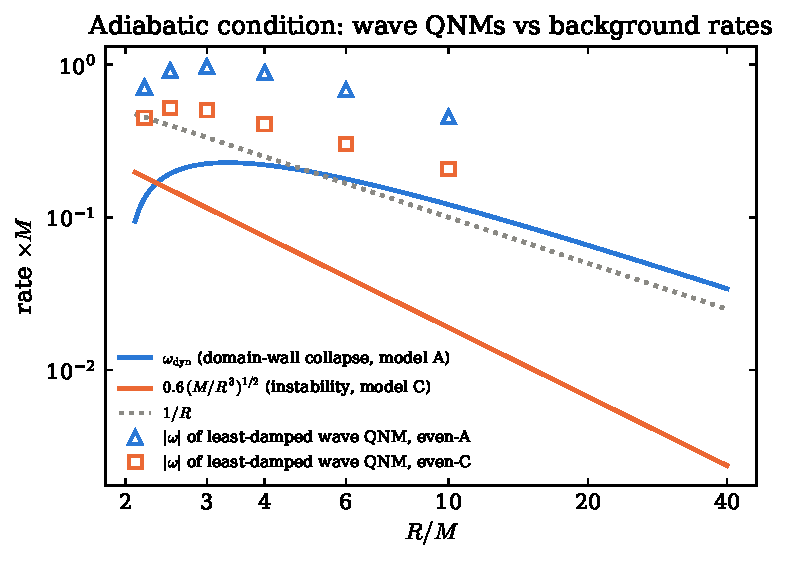
\includegraphics[width=0.6\textwidth]{r2_fig4_timescales.pdf}
\caption{Background rates versus the least-damped wave QNMs ($\ell=2$; second-round figure).}\label{fig:timescales}
\end{figure}

\subsection{Time normalization: the interior blueshift}\label{sec:blueshift}
At a static shell, continuity of $h_{ab}$ requires $\dd T=\sq\,\dd t$ (Poisson's interior metric 3.75). A
perturbation $\propto e^{-i\omega t}$ outside is therefore $\propto e^{-i\nu T}$ inside, with
\begin{equation}
\nu=\omega/\sq .
\label{eq:nu}
\end{equation}
The regular interior solution is $\jh(\nu r)$, not $\jh(\omega r)$ as in the prior notes and the task statement.
PSP26 use the same normalization, $w=F^{-1/2}\omega$. It is convenient to introduce a global tortoise coordinate
\begin{equation}
x=r_*=r+2M\ln(r/2M-1)\ (r>R),\qquad x=r_*(R)+(r-R)/\sq\ (r<R),
\label{eq:x}
\end{equation}
in which both regions obey $-\partial_t^2\Psi+\partial_x^2\Psi-V\Psi=0$, with $V_{\rm int}=f_R\,\ell(\ell+1)/r^2$
(Fig.~\ref{fig:pot}).

\begin{figure}[t]\centering
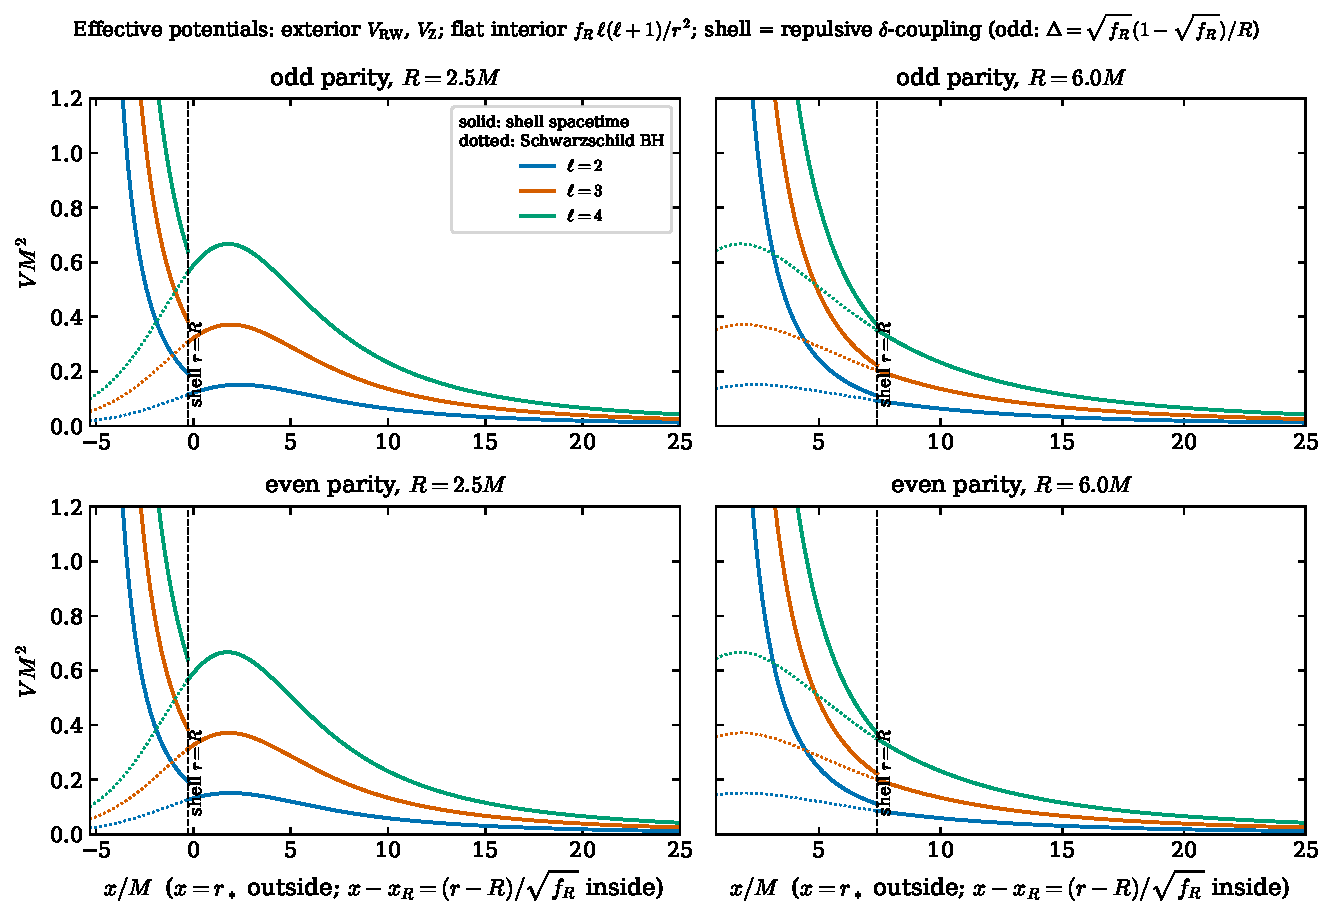
\includegraphics[width=0.95\textwidth]{fig01_potentials.pdf}
\caption{Effective potentials in the global tortoise coordinate for $\ell=2,3,4$ (first-round figure). Exterior:
$V_{\rm RW}$ and $V_{\rm Z}$. Interior: $f_R\ell(\ell+1)/r^2$. Dotted curves: the Schwarzschild continuation.}\label{fig:pot}
\end{figure}

%===============================================================================================
\section{Perturbation equations}\label{sec:pert}
We follow Martel and Poisson \cite{MP05} [MP05]. The odd harmonics are $X_A=-\varepsilon_A{}^BD_BY$ and
$X_{AB}=-\tfrac12(\varepsilon_A{}^CD_B+\varepsilon_B{}^CD_A)D_CY$. The even ones are $Y_A=D_AY$ and
$Y_{AB}=[D_AD_B+\tfrac12\ell(\ell+1)\Omega_{AB}]Y$ (MP05 3.1--3.7). We write $\lambda=\ell(\ell+1)$ and
$\mu=(\ell-1)(\ell+2)$, and we use Regge--Wheeler gauge \emph{on each side separately}: $h_2=0$ in the odd sector,
$j_a=G=0$ in the even sector \cite{RW57,MP05}.

\subsection{Odd parity}
With $p_{aB}=h_aX_B$, $h_a=(h_t,h_r)$ (MP05 5.2), the Cunningham--Price--Moncrief function \cite{CPM78}
\begin{equation}
\Psi_{\rm odd}=\frac{2r}{\mu}\Big(\partial_rh_t-\partial_th_r-\frac2rh_t\Big)
\label{eq:cpm}
\end{equation}
(MP05 5.13) obeys the Regge--Wheeler equation (MP05 5.14--5.15; RW57 Eq.~25)
\begin{equation}
\frac{\dd^2\Psi}{\dd r_*^2}+\big[\omega^2-V_{\rm RW}\big]\Psi=0,\qquad V_{\rm RW}=f\Big[\frac{\lambda}{r^2}-\frac{6M}{r^3}\Big].
\label{eq:RW}
\end{equation}
In vacuum the field equations can be inverted:
\begin{equation}
h_t=\frac f2\,\partial_r(r\Psi_{\rm odd}),\qquad h_r=\frac{r}{2f}\partial_t\Psi_{\rm odd}=-\frac{i\omega r}{2f}\Psi_{\rm odd}.
\label{eq:oddrecon}
\end{equation}
The second relation is MP05's (5.18), $\Psi_{\rm RW}=\tfrac12\partial_t\Psi_{\rm odd}$ in vacuum. The first follows
from the gauge-invariant equation $\nabla_ah^a=0$ (MP05 5.9).

\subsection{Even parity}
With $h_{tt}=fH_0$, $h_{tr}=H_1$, $h_{rr}=H_2/f$ and $p_{AB}=r^2K\Omega_{AB}Y$, the trace-free angular equation gives
$H_0=H_2\equiv H$. The Zerilli--Moncrief function \cite{Moncrief74,MP05},
\begin{equation}
\Psi_{\rm even}=\frac{2r}{\lambda}\Big[K+\frac{2f}{\Lambda}\big(H-rK'\big)\Big],\qquad \Lambda=\mu+\frac{6M}{r},
\label{eq:zm}
\end{equation}
obeys Eq.~\eqref{eq:RW} with the Zerilli potential (Zerilli Eq.~5; $f\times$MP05 4.26)
\begin{equation}
V_{\rm Z}=f\,\frac{2n^2(n+1)r^3+6n^2Mr^2+18nM^2r+18M^3}{r^3(nr+3M)^2},\qquad n=\mu/2 .
\label{eq:VZ}
\end{equation}
The linearized Einstein equations give a first-order system for $(K,H,H_1)$ plus an algebraic identity (Zerilli 1970,
p.~737). Inverting Eq.~\eqref{eq:zm} with them gives the reconstruction
\begin{align}
K&=f\,\Psi'+\frac{\mu(\mu+2)r^2+6\mu Mr+24M^2}{2r^2(\mu r+6M)}\,\Psi,\label{eq:Krec}\\
H_1&=-i\omega\Big[r\,\Psi'+\frac{\mu r^2-3\mu Mr-6M^2}{(r-2M)(\mu r+6M)}\,\Psi\Big],\\
H&=f\,\frac{\mu r^2-3\mu Mr-6M^2}{(r-2M)(\mu r+6M)}\,\Psi'+\Big[\frac{Q(r)}{2r^2(r-2M)(\mu r+6M)^2}-\frac{\omega^2r}{f}\Big]\Psi,
\label{eq:Hrec}\\
Q(r)&=\mu^2(\mu+2)r^4-2M\mu^2(\mu-1)r^3-12M^2\mu(\mu-3)r^2-72M^3(\mu-1)r-144M^4.\nonumber
\end{align}

\paragraph{How these relations were established.} Nothing in this section was copied from the literature. It was
re-derived by brute force. The symbolic code linearizes the Einstein tensor for a generic axisymmetric harmonic with
$\lambda$ symbolic, reduces the angular dependence with the Legendre equation, and eliminates $\Psi''$ with the master
equation. The residuals of all six even-parity field equations vanish identically in exact rational arithmetic at
random rational points, and so do the five odd-parity ones. Equation~\eqref{eq:zm} returns $\Psi$, and $V_{\rm Z}$
equals $f$ times MP05's (4.26).

\subsection{Chandrasekhar transformation}
The map \cite{Chandrasekhar83,Pani09}
\begin{equation}
Z=\Big[\mu(\mu+2)+\frac{72M^2f}{r(\mu r+6M)}\Big]\Psi_{\rm RW}+12M\frac{\dd\Psi_{\rm RW}}{\dd r_*}
\label{eq:chandra}
\end{equation}
takes solutions of the RW equation into solutions of the Zerilli equation for every $\omega$ (verified symbolically).
Since $\dd\Psi/\dd r_*=i\omega\Psi$ for outgoing waves, it maps $e^{i\omega r_*}$ into
$[\mu(\mu+2)+12iM\omega]e^{i\omega r_*}$. It is used to build Zerilli solutions from RW ones, and it is the reason
the two potentials share the Schwarzschild spectrum (isospectrality).

%===============================================================================================
\section{Interior solution}\label{sec:interior}
With $M=0$ both potentials reduce to $\lambda/r^2$ \cite{ondas}, so inside
\begin{equation}
\Psi''+\big[\nu^2-\lambda/r^2\big]\Psi=0\qquad(0<r<R),
\end{equation}
solved by the Riccati--Bessel functions $\jh(z)=zj_\ell(z)$ and $\yh(z)=zy_\ell(z)$ with $z=\nu r$
\cite{AS72,DLMF,ondas}. Regularity at the centre selects
\begin{equation}
\Psi_{\rm int}=A\,\jh(\nu r),\qquad \jh(z)\simeq\frac{z^{\ell+1}}{(2\ell+1)!!}\quad(z\to0).
\label{eq:intsol}
\end{equation}
Both parities have the same interior profile and differ only through the junction conditions. For the open-interior
scattering problem of Sec.~\ref{sec:scatt} we also need the Riccati--Hankel functions
$\hat h^{\rm out/in}_\ell=-\yh\pm i\jh\sim e^{\pm i(z-\ell\pi/2)}$. With the Wronskian $\jh\yh'-\jh'\yh=1$ (DLMF
10.50.1) one has ${\rm Im}(\hat h^{\rm in*}\hat h^{\rm in\prime})=-1$. The reconstruction formulas of
Sec.~\ref{sec:pert} hold inside with $M=0$ and $\omega\to\nu$, because the interior is written in its own time $T$.

%===============================================================================================
\section{Linearized junction conditions}\label{sec:junction}
\subsection{Method}
On each side the bulk perturbation is written in that side's own RW gauge. RW gauge fixes the bulk gauge
freedom completely for $\ell\ge2$, but it is not adapted to the shell: in the two gauges the shell sits at different
perturbed positions. The world-tube is therefore described by a perturbed embedding on each side (cf.\ Pani et al.\
\cite{Pani09}, Sec.~III.C and App.~A):
\begin{equation}
x^\mu_\pm(y)=X^\mu_{0\pm}(y)+\epsilon\,Z^\mu_\pm(y),\qquad Z_+=(0,\ \xi_+Y,\ 0,\ 0),\qquad
Z_-=(\zeta Y,\ \xi_-Y,\ \eta\,\partial_\theta Y,\ 0)\ [+\ \chi X^\phi\ \text{(odd)}].
\label{eq:embed}
\end{equation}
The intrinsic coordinates are chosen to coincide with the exterior ones. $\xi_\pm$ are the radial displacements of
the shell in the two gauges, and $\zeta,\eta,\chi$ describe the relative identification of time and angles. The unit
normal is solved to first order from $n_\mu e^\mu_a=0$ and $g^{\mu\nu}n_\mu n_\nu=1$. The induced metric and
Eq.~\eqref{eq:Kab} are expanded to $O(\epsilon)$, including the displacement of the background fields,
$Q(X_0+\epsilon Z)=Q(X_0)+\epsilon Z^\mu\partial_\mu Q$. The result is projected onto harmonics, and the bulk
functions are replaced by master functions through Eqs.~\eqref{eq:oddrecon}--\eqref{eq:Hrec}. The shell matter is
perturbed as $\sigma\to\sigma+\delta\sigma\,Y$, $p\to p+v_s^2\delta\sigma Y$, with $u_A=U\,D_AY$ (even) or $U\,X_A$
(odd). For the wall, $\delta S_{ab}=-\sigma\,\delta h_{ab}$. The junction conditions~\eqref{eq:israel} then become a
linear system
\begin{equation}
\mathsf A(\omega)\,\bm x=\mathsf B(\omega)\binom{\Psi_-(R)}{\Psi_-'(R)},\qquad
\bm x=(\text{shell variables},\ \Psi_+(R),\ \Psi_+'(R)),
\label{eq:linsys}
\end{equation}
whose last two components define the transfer matrix, $(\Psi_+,\Psi_+')^{\rm T}=\mathsf T(\Psi_-,\Psi_-')^{\rm T}$.

\subsection{Odd parity}\label{sec:odd}
Odd perturbations do not move the shell radially. Since $g^{rr}$ is unperturbed, $n_\alpha=f^{-1/2}\partial_\alpha r$
stays exact at first order, so $K_{ab}=-N\Gamma^r{}_{ab}$ with $N=f^{-1/2}$. The first-order Christoffel symbols
are $\delta\Gamma^r{}_{tA}=\tfrac f2(\partial_th_r-\partial_rh_t)X_A$ (the connection terms of the three covariant
derivatives cancel in pairs) and $\delta\Gamma^r{}_{AB}=fh_rX_{AB}$ (using $D_AX_B+D_BX_A=2X_{AB}$). Hence
\begin{equation}
\delta K_{tA}=\frac{\sqrt f}{2}\big(\partial_rh_t-\partial_th_r\big)X_A,\qquad \delta K_{AB}=-\sqrt f\,h_r\,X_{AB}.
\label{eq:dKodd}
\end{equation}
The first of these is Eq.~(12) of the prior notes \cite{burbuja}. By Eq.~\eqref{eq:cpm},
$\partial_rh_t-\partial_th_r=\mu\Psi/(2r)+2h_t/r$. In proper time on $\Sigma$ ($e_\tau=f_R^{-1/2}\partial_t$ outside,
$\partial_T$ inside), with the common quantity $\mathcal H=\delta h_{\tau A}$,
\begin{equation}
\text{outside: }\mathcal H=h_t^+/\sq,\ \ \delta K^+_{\tau A}=\frac{\mu\Psi_+}{4R}+\frac{\sq\,\mathcal H}{R};\qquad
\text{inside: }\mathcal H=h_T^-,\ \ \delta K^-_{\tau A}=\frac{\mu\Psi_-}{4R}+\frac{\mathcal H}{R}.
\end{equation}
Continuity of $\delta h_{AB}$ forces $\chi=0$. Three equations remain.
\begin{enumerate}
\item \emph{$AB$ Israel equation.} $\delta S^{\rm odd}_{AB}=0$ (since $\delta h_{AB}=0$ and $u_Au_B=O(\epsilon^2)$),
so $[\sq h_r]=0$. With $h_r^+=-i\omega R\Psi_+/2f$ and $h_r^-=-i\nu R\Psi_-/2$, $\nu=\omega/\sq$, this gives
$\Psi_+(R)=\Psi_-(R)$ exactly.
\item \emph{$\tau A$ Israel equation.} With $\delta S_{\tau A}=-(\sigma+p)U+p\mathcal H$ and $[K]=4\pi(2p-\sigma)$, the
left-hand side is $\mu[\Psi]/4R+(\sq-1)\mathcal H/R$, where $(\sq-1)/R=-4\pi\sigma$. This leaves
$\mu[\Psi]/4R=8\pi(\sigma+p)U$, hence $U=0$: odd perturbations do not set the shell matter in motion, in agreement
with $\partial_\tau u_A=0$ from $D_bS^{ab}=0$. The background trace $[K]^{(0)}$, flagged as ``the remaining step'' in
\cite{burbuja}, combines with the pressure term into $[K]^{(0)}-8\pi p=-4\pi\sigma$. The dependence on $p$, and with
it on $\ddot R$ for the wall, cancels identically.
\item \emph{Continuity of $\mathcal H$:} $\tfrac12(r\Psi_-)'|_R=\tfrac{\sq}2(r\Psi_+)'|_R$.
\end{enumerate}
Together:
\begin{equation}
\boxed{\ \Psi_+=\Psi_-,\qquad \sq\,\Psi_+'-\Psi_-'=\frac{1-\sq}{R}\,\Psi=4\pi\sigma\,\Psi\ }
\qquad\Longleftrightarrow\qquad\Big[\frac{\dd\Psi}{\dd\ell_{\rm p}}\Big]=4\pi\sigma\Psi,
\label{eq:oddfinal}
\end{equation}
where $\ell_{\rm p}$ is proper radial distance. In the global coordinate \eqref{eq:x}, $[\dd\Psi/\dd x]=\Delta_{\rm odd}\Psi$
with
\begin{equation}
\Delta_{\rm odd}=\frac{\sq(1-\sq)}{R}=4\pi\sigma\sq>0 .
\label{eq:Deltaodd}
\end{equation}
The shell acts as a \emph{repulsive $\delta$-function potential} $\Delta_{\rm odd}\,\delta(x-x_R)$, independent of
$\omega$ and of the equation of state. The transfer matrix is
$\mathsf T_{\rm odd}=\begin{pmatrix}1&0\\(1-\sq)/(R\sq)&1/\sq\end{pmatrix}$, with $\det\mathsf T_{\rm odd}=f_R^{-1/2}$.
The same condition follows from the brute-force symbolic system, for model C (4 equations, 4 unknowns) and for
model A (4 equations, 3 unknowns, consistent with rank 3). It agrees with PSP26 Eq.~(5.23),
$F^{1/2}\eta_{\rm out}-\eta_{\rm in}+F^{1/2}-1=0$ with $\eta=R\psi'/\psi$: the phase factors of their retarded-time
slicing cancel because $w=F^{-1/2}\omega$. It also agrees with Pani et al.'s (3.29) and (A35), $[h_0]=0$ and
$[\sqrt h\,h_1]=0$, and it reduces to the identity (continuity of $\Psi$ and $\Psi'$, the ``inviscid'' limit of
Boyanov et al.\ \cite{Boyanov25}) as $M\to0$.

\begin{verifbox}
The second round derived the same result by a completely independent route (companion report and
App.~\ref{app:axial}). Linearizing the Einstein equations for axial perturbations of a smooth, static,
\emph{anisotropic} fluid gives the master potential
$V=e^{2\Phi}[\ell(\ell+1)/r^2-6m/r^3+4\pi(\rho-p_r)]$. It generalises the familiar stellar result of Chandrasekhar
and Ferrari \cite{ChandrasekharFerrari91}; see also \cite{ThorneCampolattaro67,Kojima92}. For a shell with $p_r=0$ the
$4\pi\rho$ term becomes $\Delta_{\rm odd}\,\delta(x-x_R)$, which is exactly Eq.~\eqref{eq:Deltaodd}. A numerical
thick-shell computation converges linearly in the thickness to the junction \eqref{eq:oddfinal} and to none of the
alternatives tried (Fig.~\ref{fig:thick}).
\end{verifbox}

\begin{figure}[t]\centering
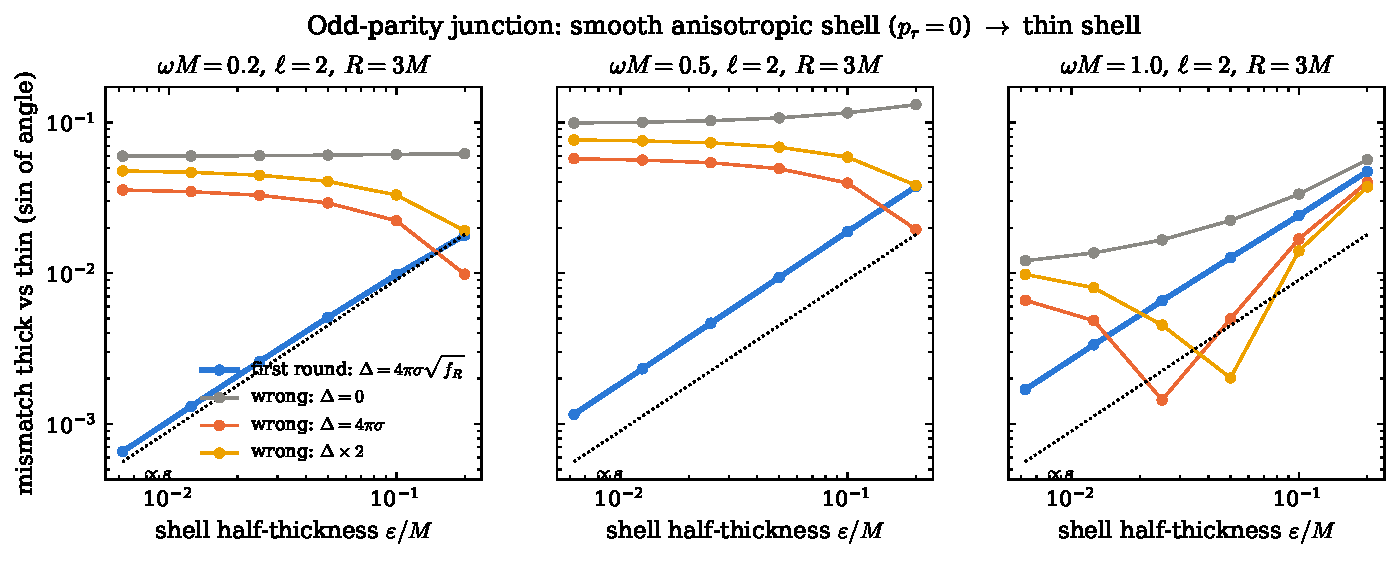
\includegraphics[width=\textwidth]{r2_fig1_thick_shell_limit.pdf}
\caption{Thick-shell test of the odd junction (second round): mismatch between a smooth anisotropic shell of
half-thickness $\varepsilon$ and the thin-shell prediction.}\label{fig:thick}
\end{figure}

\subsection{Even parity}\label{sec:even}
\paragraph{Induced metric.} The first-order induced metric from the two sides is (coefficients of $Y$, $D_AY$,
$\Omega_{AB}Y$ and $Y_{AB}$)
\begin{align}
\text{outside:}&\quad \delta h_{\tau\tau}=H_+-\tfrac{2M}{R(R-2M)}\xi_+,\qquad \delta h_{\tau A}=0,\nonumber\\
&\quad \delta h^{\rm tr}_{AB}=R^2K_++2R\xi_+,\qquad \delta h^{\rm tf}_{AB}=0,\nonumber\\
\text{inside:}&\quad \delta h_{\tau\tau}=H_-+2i\nu\zeta,\qquad \delta h_{\tau A}=-\zeta-i\nu R^2\eta,\nonumber\\
&\quad \delta h^{\rm tr}_{AB}=R^2K_--\lambda R^2\eta+2R\xi_-,\qquad \delta h^{\rm tf}_{AB}=2R^2\eta .
\end{align}
The first junction condition forces $\eta=\zeta=0$ and leaves
$H_+-\frac{2M}{R(R-2M)}\xi_+=H_-$ and $RK_++2\xi_+=RK_-+2\xi_-$, in agreement with Pani et al.'s (A16), (A20). Because
$\xi_+\ne\xi_-$, the shell's radial displacement is different in the two RW gauges. This is why the even sector
cannot reduce to a scalar jump condition.

\paragraph{Israel equations.} The four even components ($\tau\tau$, $\tau A$, trace and trace-free $AB$) of
$[\delta K_{ab}-\delta h_{ab}K-h_{ab}\delta K]=-8\pi\delta S_{ab}$ involve $H_\pm,H'_\pm,K_\pm,K'_\pm,H_{1\pm},\xi_\pm$ and
the matter variables. For model C,
\begin{equation}
\delta S_{\tau\tau}=\delta\sigma-\sigma\delta h_{\tau\tau},\quad \delta S_{\tau A}=-(\sigma+p)U+p\,\delta h_{\tau A},\quad
\delta S^{\rm tr}_{AB}=v_s^2\delta\sigma R^2+p\,\delta h^{\rm tr}_{AB},\quad \delta S^{\rm tf}_{AB}=p\,\delta h^{\rm tf}_{AB}.
\end{equation}
Model C gives 8 equations for the 8 unknowns $(\xi_+,\xi_-,\zeta,\eta,\delta\sigma,U,\Psi_+,\Psi_+')$, with full rank.
Its solution defines $\mathsf T^{\rm C}_{\rm even}(\omega;\ell,R/M,\Gamma)$.

\paragraph{Structure of the result.}
\begin{itemize}
\item $\Psi$ is \emph{discontinuous}. $\mathsf T_{\rm even}$ is a full $2\times2$ matrix that depends on frequency
(through the $\omega^2$ term of $H$ and through the shell's inertia) and, through $v_s^2$, on the shell's equation of
state. The even problem is a genuine $2\times2$ matching, as the task statement anticipated might happen.
\item $\det\mathsf T^{\rm C}_{\rm even}=f_R^{-1/2}$ exactly, and $\mathsf T$ is real for real $\omega$, so the flux is
conserved: this is the identity that makes $\RR+\TT=1$ (Sec.~\ref{sec:scatt}). It is \emph{not} built into the
construction, so it is a strong test.
\item $\mathsf T_{\rm even}\to\mathbb I$ as $M\to0$ at fixed $R$ (linearly in $M$).
\item The matrix has poles on the matter scale $\omega\sim(M/R^3)^{1/2}$, which the odd sector lacks. They signal
the shell's own oscillations.
\end{itemize}
\paragraph{High-precision arithmetic.} The exact matrices involve large cancellations near $R=2M$. In double
precision $\det\mathsf T\sq-1$ is $\sim10^{-7}$ at $2.2M$ and the method fails below $\simeq2.05M$. For $R<2.3M$ the
system is therefore solved with 40-digit \texttt{mpmath}, and $\det\mathsf T\sq=1$ then holds to $10^{-15}$ down to
$2.01M$.

\begin{verifbox}
The second round verified $\det\mathsf T\sq=1$ to $1.1\times10^{-12}$ over 300 random real and complex parameter
sets, the reality of $\mathsf T$, flux conservation to $10^{-13}$, and linear convergence to $\mathbb I$ as $M\to0$. It
also regenerated the symbolic matrices from the script and found them identical. The poles lie at
$\omega(R^3/M)^{1/2}\approx1.54$ and $0.985i$ ($R=6M$): on the matter scale, but not at the matter QNMs themselves.
\end{verifbox}

\subsection{Model A: an adiabatic matching and its limits}\label{sec:evenA}
For an exact solution of the moving-shell problem, the $\tau\tau$ and $\tau A$ Israel equations follow from the
others through the Codazzi identity and $D_bS^{ab}=0$. That is why the overdetermined odd system of model A is
consistent. In the even sector the frozen, monochromatic ansatz is not an exact solution at the turning point:
$\dot T_0=\beta/f$ has $\ddot T_0=0$ but $\dddot T_0\propto\ddot R^2\ne0$. Correspondingly ${\rm rank}\,\mathsf A=6$
while ${\rm rank}[\mathsf A|\mathsf B]=8$. The first round imposed the four metric-continuity equations and the two
angular Israel equations (called ``evolution'' equations) and monitored the $\tau\tau$ and $\tau A$ rows
(``constraints''). The constraint violation then decreases as $\omega^{-1}$, and $|\RR+\TT-1|$ decreases as
$\omega^{-2}$ (Figs.~\ref{fig:energy} and \ref{fig:modelA1}).

\begin{verifbox}
For a frozen ansatz that is not a solution, the choice of which two of the four Israel equations to impose is a
\emph{prescription}. The second round kept metric continuity and tried all six choices
(Fig.~\ref{fig:modelA2}). The resulting reflectivities differ at $O(1)$ even at $\omega M=30$, from total reflection
to the $\delta$-barrier law, and the lowest QNMs differ by 20--30\%. With the first round's choice the energy error is
\emph{larger than $\RR$ itself} at all high frequencies. The choice ``$\tau\tau$ + trace-free'' conserves energy exactly
and reproduces the universal high-frequency law of the odd sector and of model C. The even-parity results of
model A are therefore \emph{not} an $O(\omega_{\rm dyn}/\omega)$-accurate approximation. They should be regarded as
undetermined by the frozen-background idealization. The odd sector of model A is unaffected.
\end{verifbox}

\begin{figure}[t]\centering
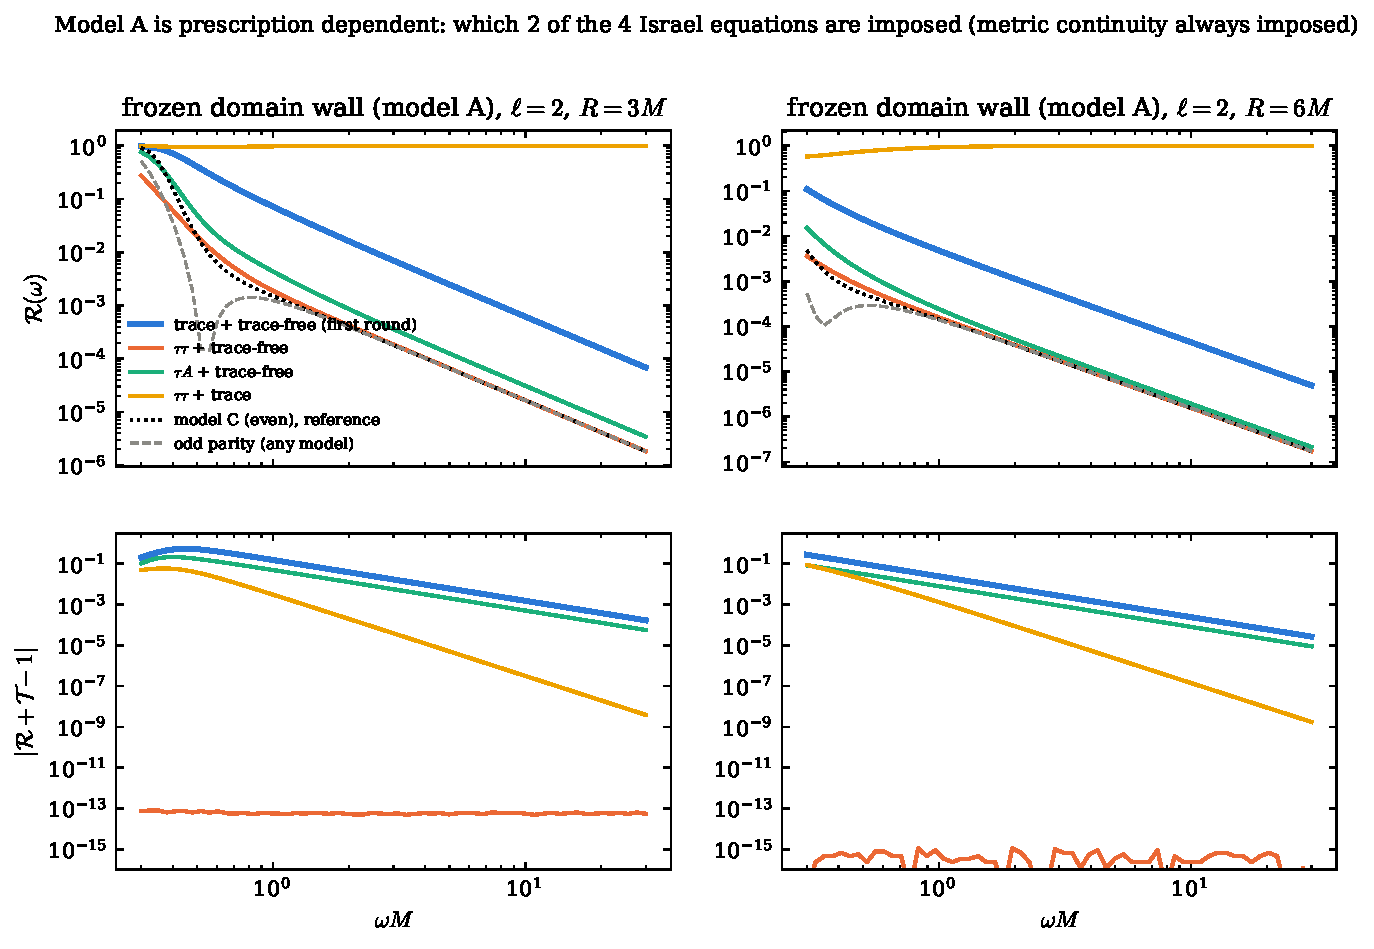
\includegraphics[width=\textwidth]{r2_fig3_modelA_prescriptions.pdf}
\caption{Reflectivity and energy balance of the frozen domain wall for four admissible prescriptions (second
round). The first-round prescription is the thick blue curve.}\label{fig:modelA2}
\end{figure}

%===============================================================================================
\section{The scattering problem}\label{sec:scatt}
\subsection{Definitions}
The interior is regular and nothing is absorbed, so the physical (closed) system reflects everything. Outside,
$\Psi_+\to B_{\rm in}e^{-i\omega r_*}+B_{\rm out}e^{+i\omega r_*}$ with $|B_{\rm out}/B_{\rm in}|=1$ for real $\omega$,
so $S=B_{\rm out}/B_{\rm in}=e^{2i\delta(\omega)}$, and the QNMs appear as resonances of the phase $\delta$. The same is
true for the inviscid star of Boyanov et al.\ \cite{Boyanov25}, whose $\RR^2=1$ in that limit. To obtain non-trivial
coefficients we treat the \emph{exterior potential plus shell} as a scatterer between infinity and an ``open''
interior that contains only the ingoing wave $\Psi_-=\hat h^{\rm in}_\ell(\nu r)$. We then define
\begin{equation}
\RR(\omega)=\Big|\frac{B_{\rm out}}{B_{\rm in}}\Big|^2,\qquad \TT(\omega)=\frac1{|B_{\rm in}|^2}.
\label{eq:RT}
\end{equation}
The Wronskian flux $J={\rm Im}(\Psi^*\partial_x\Psi)$ is constant on each side: $J_{\rm int}=\sq\,\nu\,{\rm Im}(\hat h^{\rm in*}\hat h^{\rm in\prime})=-\omega$
and $J_{\rm ext}=\omega(|B_{\rm out}|^2-|B_{\rm in}|^2)$. If the junction conserves $J$, then $\RR+\TT=1$. For a real
$\mathsf T$ this is the statement $\det\mathsf T=f_R^{-1/2}$. This definition is a physically motivated convention:
it describes waves that, once through the shell, never return. It is the analogue of the horizon boundary condition
of a black hole, and it makes the black-hole limit transparent.

\subsection{Limits}
\begin{itemize}
\item $\omega\to0$: $\RR\to1$. The irregular static branch $r^{-\ell}$ of the interior Hankel function dominates, and
the matched exterior solution is a standing wave (the shell's tidal response). Long waves do not see the shell, as
for the star of Boyanov et al.
\item $R\to2M$: $\RR\to\RR_{\rm BH}$. The shell sits deep in the near-horizon region, where $V\to0$ and
$\Delta_{\rm odd}\to0$, so the transmitted wave is exactly the horizon-ingoing one of Vishveshwara's problem
\cite{Vishveshwara70}.
\item $M\to0$: $\RR\to0$ (flat space).
\item High frequency. The potentials are negligible and only the $\delta$ barrier remains. With
$\Psi=e^{-i\omega x}+re^{i\omega x}$ outside and $te^{-i\omega x}$ inside, continuity and
$[\Psi']=\Delta\Psi$ give $r=\Delta/(2i\omega-\Delta)$, so
\begin{equation}
\RR\simeq\frac{\Delta_{\rm odd}^2}{4\omega^2+\Delta_{\rm odd}^2}.
\label{eq:deltalaw}
\end{equation}
No impedance mismatch arises, because the local wavenumber $\omega/\sq$ in proper distance is continuous across the
shell. The thin shell becomes \emph{transparent} at high frequency, unlike the viscous star of Boyanov et al., which
absorbs.
\end{itemize}

%===============================================================================================
\section{Numerical methods}\label{sec:num}
\subsection{Method 1: transfer matrix with a continued-fraction exterior basis}
The purely outgoing exterior solution is expanded about a point $r=R_2$ \cite{LNS93,Pani09}:
\begin{equation}
\Psi_{\rm up}=\chi(r)\sum_{n\ge0}a_nz^n,\qquad z=1-\frac{R_2}{r},\qquad \chi=(r-2M)^{2iM\omega}e^{i\omega r}.
\end{equation}
The identity $f\chi'/\chi=i\omega$ turns Eq.~\eqref{eq:RW} into $c(z)\phi''+d(z)\phi'+e(z)\phi=0$ with $u=1-z$ and
$m=M/R_2$:
\begin{equation}
c=u^2(1-2mu),\quad d=-2u+6mu^2+2i\omega R_2,\quad e=6mu-\lambda .
\end{equation}
This is Pani et al.'s (B4) with $\omega\to-\omega$ (they use $e^{+i\omega t}$). Writing $c=\sum c_jz^j$ etc., the
coefficients obey the four-term recurrence
$\alpha_na_{n+1}+\beta_na_n+\gamma_na_{n-1}+\delta_na_{n-2}=0$, with $\alpha_n=n(n+1)c_0$,
$\beta_n=n(n-1)c_1+nd_0$, $\gamma_n=(n-1)(n-2)c_2+(n-1)d_1+e_0$, $\delta_n=(n-2)(n-3)c_3+(n-2)d_2+e_1$. Gaussian
elimination reduces it to three terms \cite{Leaver90} (Pani's B10--B13). The minimal solution \cite{Gautschi67} is
then selected by the continued fraction
$a_1/a_0=-\hat\gamma_1/(\hat\beta_1-\hat\alpha_1\hat\gamma_2/(\hat\beta_2-\dots))$ (B17), whose depth is doubled until it
converges to $10^{-12}$. Then $\Psi_{\rm up}'/\Psi_{\rm up}|_{R_2}=i\omega R_2/(R_2-2M)+(a_1/a_0)/R_2$. The series must
converge for $0\le z<1$, so the singular point $r=2M$, at $z=1-R_2/2M$, must lie outside the unit disk: $R_2\ge4M$
(Pani's ``$R_2>2$'' in units $2M=1$). The code uses $R_2=\max(R,4.5M)$ and integrates from $R_2$ down to $R$ when
needed. Zerilli solutions follow from Eq.~\eqref{eq:chandra}. For real $\omega$, $\Psi_{\rm in}=\Psi_{\rm up}^*$, and the
normalization $|\Psi_{\rm up}(R)|^2=\omega/{\rm Im}(\partial_{r_*}\ln\Psi_{\rm up})$ follows from the Wronskian.

\subsection{Method 2: shooting}
The exterior equation is integrated outward in $r$ from $R^+$ to $r_{\rm far}=\max(150M,60/\omega)$ with DOP853
\cite{Hairer93,SciPy20} (\texttt{rtol}$=10^{-10}$, \texttt{atol}$=10^{-12}$). At $r_{\rm far}$ the solution is projected on
$\Psi_{\rm up}=e^{i\omega r_*}\sum_kc_kr^{-k}$ and $\Psi_{\rm up}^*$, whose coefficients follow from
$fu''+(f'+2i\omega)u'-(\lambda/r^2-6M/r^3)u=0$:
\begin{equation}
2i\omega(k+1)c_{k+1}=[k(k+1)-\lambda]c_k-2M(k^2-4)c_{k-1},\qquad c_0=1 .
\label{eq:asym}
\end{equation}
The series is asymptotic and is truncated at its smallest term. The reflectivity estimator of Boyanov et al.\
(App.~B1), $|i\omega\Psi+\partial_{r_*}\Psi|/|i\omega\Psi-\partial_{r_*}\Psi|=|B_{\rm out}/B_{\rm in}|$ averaged over four
periods, is also evaluated. The two methods share only the junction matrix and the interior functions.

\subsection{Quasinormal modes}
QNMs are the zeros of the normalized Wronskian at $R^+$ between the solution coming from the regular interior
through the junction, $\bm y_J=\mathsf T(\omega)(\jh,\nu\jh')$, and the outgoing solution:
$W=(\Psi_J\Psi_{\rm up}'-\Psi_J'\Psi_{\rm up})/(|\bm y_J||\bm y_{\rm up}|)$. Method 1 takes $\Psi_{\rm up}$ from the
continued fraction. Method 2 follows the inward strategy of Boyanov et al.: it starts from the asymptotic series at a
far point on the complex ray $r=R+se^{i\varphi}$, $\varphi=\pi/2-\arg\omega$, along which $\Psi_{\rm up}$ is
exponentially subdominant, and integrates back to $R$. Candidates come from scans of $\log|W|$ in the complex plane,
with extra scans near the real axis for compact shells and post-Newtonian seeds (PSP26 Eq.~7.8) for the matter modes.
They are refined with \texttt{scipy.optimize.root}, and every root is re-converged with Method 2.

\subsection{Schwarzschild black hole and WKB}
Black-hole QNMs come from Leaver's continued fraction \cite{Leaver85} (units $2M=1$, $\rho=-i\omega$,
$\alpha_n=n^2+(2\rho+2)n+2\rho+1$, $\beta_n=-[2n^2+(8\rho+2)n+8\rho^2+4\rho+\ell(\ell+1)-3]$,
$\gamma_n=n^2+4\rho n+4\rho^2-4$), with inversion index equal to the overtone number. The black-hole reflectivity
follows from integration from $r=2M(1+10^{-6})$ with a Frobenius start. The WKB QNM formula of arbitrary order is
obtained from the equivalent perturbative (Bender--Wu \cite{BenderWu69}) expansion of an inverted anharmonic
oscillator \cite{Hatsuda20}, computed with symbolic overtone $n$ through the hypervirial--Hellmann--Feynman recursion
\cite{Killingbeck78,FernandezCastro87},
\begin{equation}
2kE\langle x^{k-1}\rangle=2k\langle x^{k-1}V\rangle+\langle x^kV'\rangle-\tfrac12k(k-1)(k-2)\langle x^{k-3}\rangle,
\end{equation}
with the $r_*$-derivatives of $V$ at its maximum. Truncation after $g^{2(N-1)}$ reproduces the $N$-th order formula:
Schutz--Will \cite{SW85} for $N=1$, Iyer--Will \cite{IW87,Iyer87} for $N=3$, Konoplya \cite{Konoplya03} for $N=6$.
For modes trapped between the flat interior and the exterior barrier of ultracompact shells, the WKB estimate is a
Bohr--Sommerfeld condition with Langer's replacement $\lambda\to(\ell+\frac12)^2$ \cite{Langer37},
\begin{equation}
\int_{r_1}^{R}\!\sqrt{\nu^2-\tfrac{(\ell+1/2)^2}{r^2}}\,\dd r+\int_R^{r_a}\!\sqrt{\omega^2-V}\,\frac{\dd r}{f}=\pi(n+\tfrac12),
\end{equation}
plus Gamow tunnelling,
${\rm Im}\,\omega=-T_b/(4\omega\int\dd x/\sqrt{\omega^2-V})$ with $T_b=\exp(-2\int_{r_a}^{r_b}\sqrt{V-\omega^2}\,\dd r/f)$.

%===============================================================================================
\section{Results}\label{sec:results}
\subsection{Validation}
\begin{table}[h]\centering\small
\caption{Validation summary of the first round (M1/M2: transfer-matrix and shooting methods; $|\Delta_{12}|$: maximum
difference over $\omega M\in[0.005,2]$).}\label{tab:valid}
\resizebox{\textwidth}{!}{\begin{tabular}{lr}\toprule
Check & value\\\midrule
Odd: generated vs analytic $\mathsf T$ & 5.7e-16 \\
Odd: $\mathsf T^{\rm A}-\mathsf T^{\rm C}$ & 1.1e-15 \\
Even C: $|\mathsf T-\mathbb{I}|$ at $M=10^{-8}$ (transparent limit) & 4.0e-09 \\
Even A: $|\mathsf T-\mathbb{I}|$ at $M=10^{-8}$ & 4.7e-09 \\
Even C: $\max|\det\mathsf T\,\sqrt{f_R}-1|$ & 3.6e-12 \\
Even A: constraint violation, $R=3M$, $\omega M=1$ & 1.2e-01 \\
Even A: constraint violation, $R=3M$, $\omega M=10$ & 1.4e-02 \\
Even A: constraint violation, $R=3M$, $\omega M=100$ & 1.4e-03 \\
Even A: constraint violation, $R=6M$, $\omega M=1$ & 6.0e-02 \\
Even A: constraint violation, $R=6M$, $\omega M=10$ & 7.9e-03 \\
Even A: constraint violation, $R=6M$, $\omega M=100$ & 7.9e-04 \\
odd, $\ell=2$, $R=3M$: $\max_\omega|\mathcal R+\mathcal T-1|$ (M2) / $\max|\Delta_{12}|$ / Boyanov estimator & 5.3e-10 / 5.3e-10 / 2.5e-06 \\
odd, $\ell=2$, $R=6M$: $\max_\omega|\mathcal R+\mathcal T-1|$ (M2) / $\max|\Delta_{12}|$ / Boyanov estimator & 6.0e-10 / 6.0e-10 / 2.0e-06 \\
even-C, $\ell=2$, $R=3M$: $\max_\omega|\mathcal R+\mathcal T-1|$ (M2) / $\max|\Delta_{12}|$ / Boyanov estimator & 5.3e-10 / 5.3e-10 / 4.0e-06 \\
even-C, $\ell=2$, $R=6M$: $\max_\omega|\mathcal R+\mathcal T-1|$ (M2) / $\max|\Delta_{12}|$ / Boyanov estimator & 6.1e-10 / 6.1e-10 / 3.2e-06 \\
even-A, $\ell=2$, $R=3M$: $\max_\omega|\mathcal R+\mathcal T-1|$ (M2) / $\max|\Delta_{12}|$ / Boyanov estimator & 5.4e-01 / 6.0e-10 / 2.5e-06 \\
even-A, $\ell=2$, $R=6M$: $\max_\omega|\mathcal R+\mathcal T-1|$ (M2) / $\max|\Delta_{12}|$ / Boyanov estimator & 2.2e+00 / 6.1e-10 / 3.6e-06 \\
Low frequency: $\max|1-\mathcal R|$ at $\omega M=10^{-3}$ (all models) & 8.9e-16 \\
\bottomrule\end{tabular}
}
\end{table}
\paragraph{Energy conservation.} For odd parity and for model C, $|\RR+\TT-1|\lesssim6\times10^{-10}$ over
$\omega M\in[0.005,2]$ (Fig.~\ref{fig:energy}), with $\RR$ and $\TT$ obtained independently from the asymptotic
amplitudes. For model A the violation is an error of the frozen approximation and decays as $\omega^{-2}$.
\paragraph{Consistency of the methods.} Transfer matrix and shooting agree to $\lesssim10^{-9}$ on $\RR$ and $\TT$
(Fig.~\ref{fig:tm}). On the QNMs they agree to $10^{-10}$--$10^{-13}$ for most modes, and to better than
$6.4\times10^{-5}$ for all 397 catalogued modes; the task required $10^{-4}$.
\paragraph{Pure Schwarzschild.} The exterior machinery gives $\omega M=0.3736716844-0.0889623157i$ for $\ell=2$,
$n=0$. All overtones $n\le3$ for $\ell=2,3,4$ agree with Berti, Cardoso and Starinets' tables \cite{BCS09}
(Table~\ref{tab:bhqnm}). The black-hole reflectivity is identical for RW and Zerilli to $10^{-7}$ (isospectrality) and
reproduces Vishveshwara's Fig.~2: $\RR=1.55\times10^{-2}$ at $(2M\omega)^2=1$ and $5.3\times10^{-9}$ at $(2M\omega)^2=4$.
\paragraph{WKB.} Relative errors for $\ell=2$, $n=0$ are $6.6\times10^{-2}$, $1.5\times10^{-3}$ and $2.3\times10^{-4}$ at
orders 1, 3 and 6 (Fig.~\ref{fig:wkb}). They decrease with $\ell$ and grow with $n$. The third-order values coincide
with the explicit Iyer--Will formula; e.g.\ $\ell=2$: $0.3732-0.0892i$ ($n=0$) and $0.3460-0.2749i$ ($n=1$).

\begin{table}[h]\centering\small
\caption{Schwarzschild QNMs $\omega M$: Leaver continued fraction vs WKB of orders 1, 3, 6.}\label{tab:bhqnm}
\begin{tabular}{rrllll}\toprule
$\ell$ & $n$ & Leaver CF (this code) & WKB 1st & WKB 3rd & WKB 6th\\\midrule
2 & 0 & $0.37367168-0.08896232i$ & $0.3988-0.0883i$ & $0.37316-0.08922i$ & $0.373619-0.088891i$ \\
2 & 1 & $0.34671100-0.27391488i$ & $0.4534-0.2330i$ & $0.34602-0.27492i$ & $0.346297-0.273480i$ \\
2 & 2 & $0.30105345-0.47827698i$ & $0.5170-0.3406i$ & $0.30293-0.47106i$ & $0.298520-0.477560i$ \\
2 & 3 & $0.25150496-0.70514820i$ & $0.5775-0.4268i$ & $0.24746-0.67290i$ & $0.241715-0.709595i$ \\
3 & 0 & $0.59944329-0.09270305i$ & $0.6166-0.0923i$ & $0.59927-0.09273i$ & $0.599443-0.092703i$ \\
3 & 1 & $0.58264380-0.28129811i$ & $0.6619-0.2580i$ & $0.58235-0.28141i$ & $0.582642-0.281290i$ \\
3 & 2 & $0.55168490-0.47909275i$ & $0.7251-0.3925i$ & $0.55320-0.47668i$ & $0.551594-0.479047i$ \\
3 & 3 & $0.51196191-0.69033710i$ & $0.7909-0.5038i$ & $0.51575-0.67743i$ & $0.511099-0.690468i$ \\
4 & 0 & $0.80917838-0.09416396i$ & $0.8223-0.0939i$ & $0.80910-0.09417i$ & $0.809178-0.094164i$ \\
4 & 1 & $0.79663153-0.28433435i$ & $0.8602-0.2694i$ & $0.79650-0.28437i$ & $0.796631-0.284334i$ \\
4 & 2 & $0.77270953-0.47990818i$ & $0.9187-0.4204i$ & $0.77364-0.47897i$ & $0.772695-0.479900i$ \\
4 & 3 & $0.73983673-0.68392432i$ & $0.9844-0.5492i$ & $0.74331-0.67830i$ & $0.739665-0.683902i$ \\
\bottomrule\end{tabular}

\end{table}

\begin{figure}[t]\centering
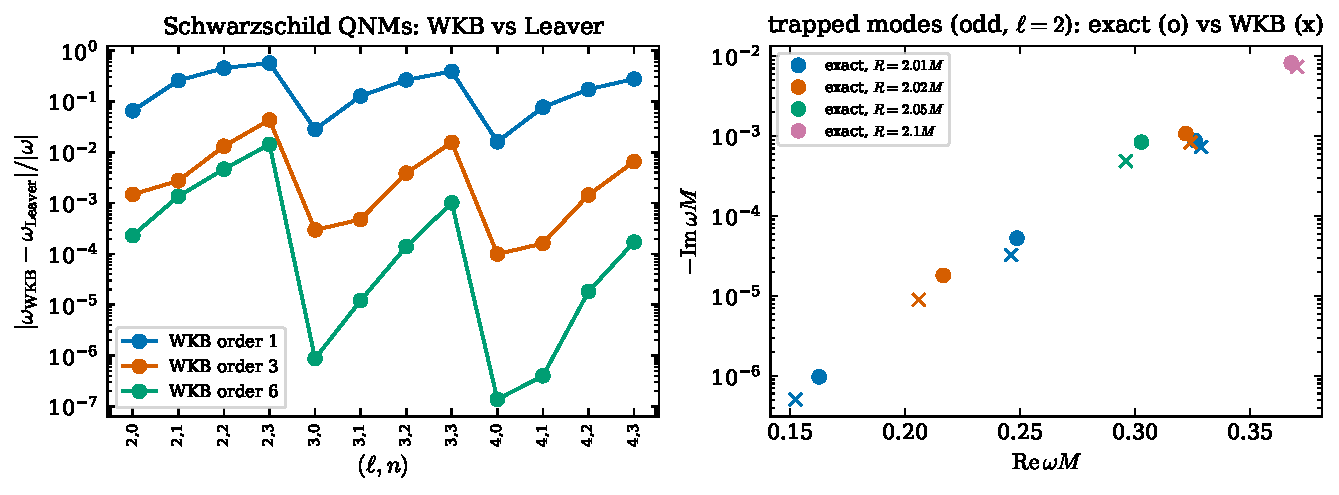
\includegraphics[width=0.95\textwidth]{fig12_wkb.pdf}
\caption{WKB validation (first round). Left: relative error of WKB orders 1, 3, 6 vs Leaver. Right: trapped modes of ultracompact shells, exact (o) vs Bohr--Sommerfeld/Gamow WKB (x).}\label{fig:wkb}
\end{figure}

\begin{figure}[t]\centering
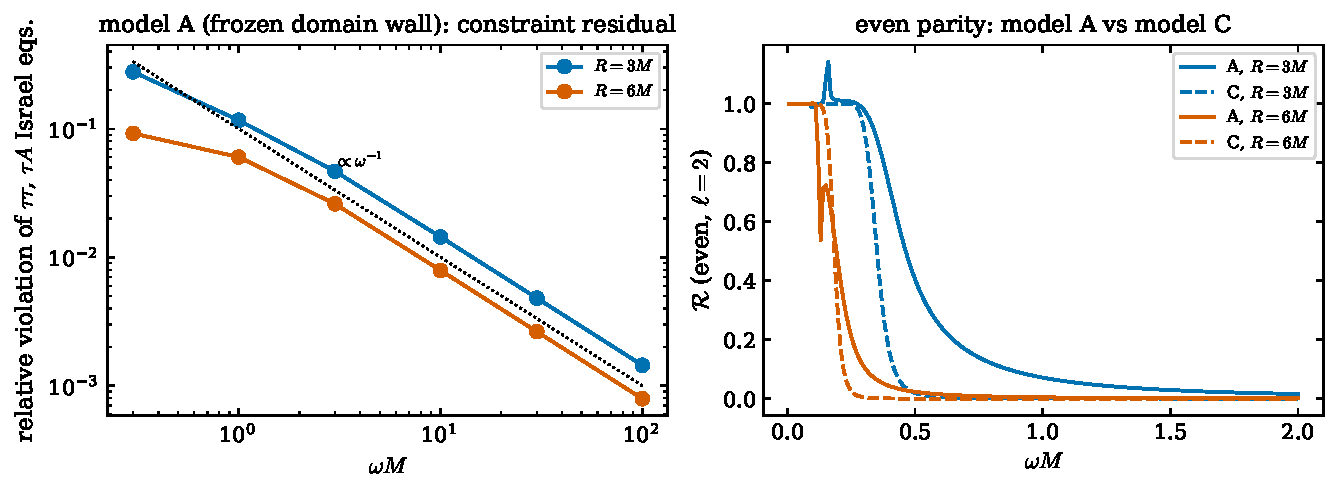
\includegraphics[width=0.95\textwidth]{fig11_modelA_adiabatic.pdf}
\caption{Model A with the first-round prescription. Left: relative violation of the $\tau\tau$ and $\tau A$ Israel equations, $\propto\omega^{-1}$. Right: even-parity reflectivity of models A and C (but see Fig.~\ref{fig:modelA2}).}\label{fig:modelA1}
\end{figure}

\begin{figure}[p]\centering
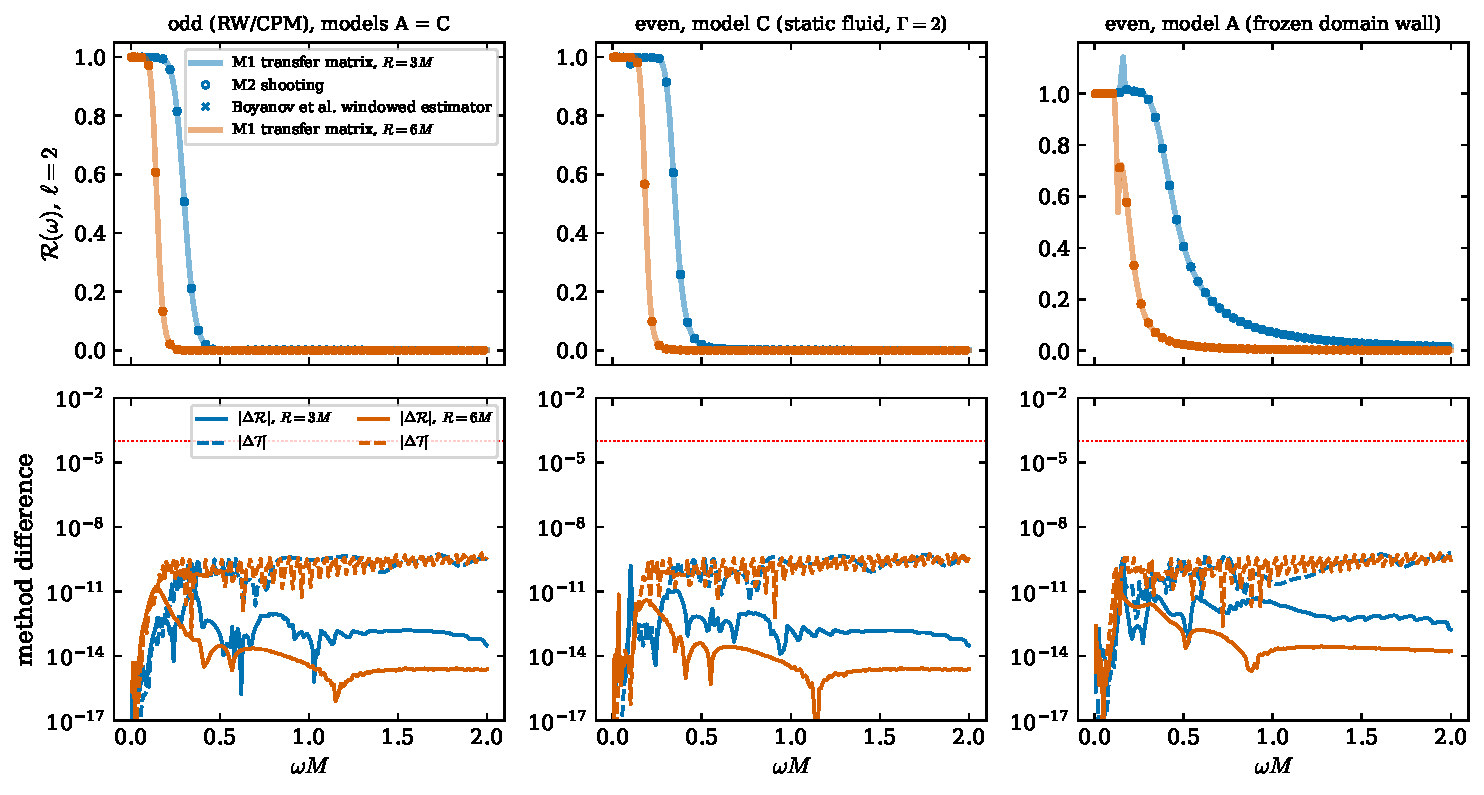
\includegraphics[width=\textwidth]{fig05_transfer_vs_shooting.pdf}
\caption{Transfer matrix (lines) vs shooting (circles). The bottom row shows the absolute differences; the red line
is the required $10^{-4}$.}\label{fig:tm}
\vspace{4mm}
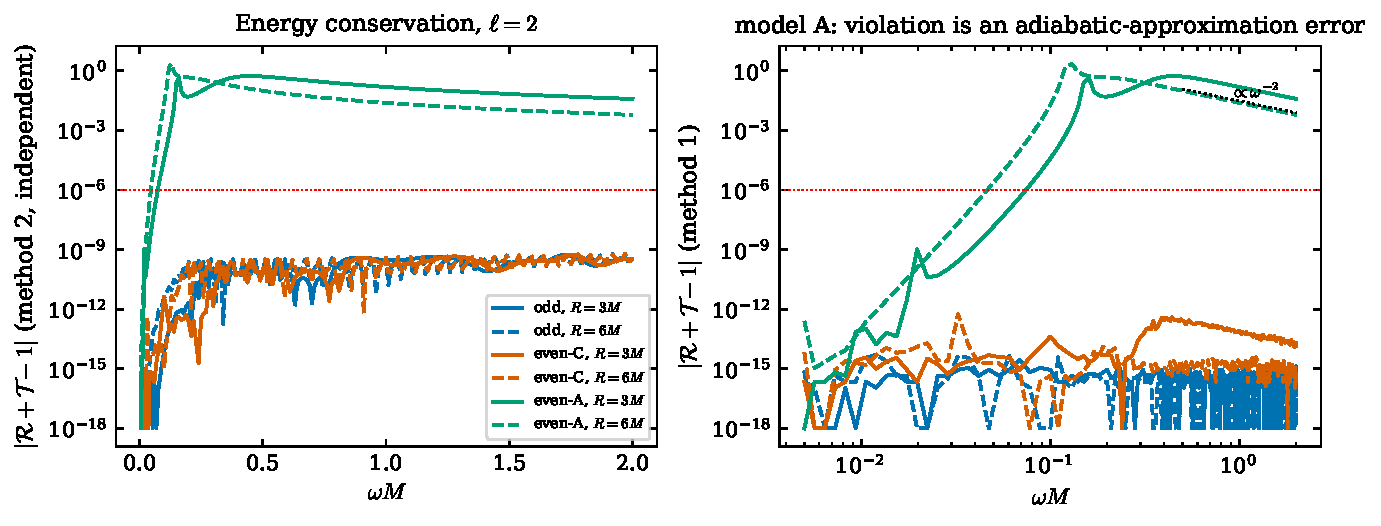
\includegraphics[width=\textwidth]{fig08_energy_conservation.pdf}
\caption{Energy conservation $|\RR+\TT-1|$. Left: Method 2. Right: Method 1 on log--log axes (model A decays as
$\omega^{-2}$).}\label{fig:energy}
\end{figure}

\subsection{Scattering coefficients}
Figures~\ref{fig:RT2}--\ref{fig:eos} show $\RR(\omega)$ and $\TT(\omega)$.
\begin{enumerate}
\item At low frequency the shell is a perfect reflector. For compact shells ($R\lesssim3M$) the transition to
transparency happens at $\omega\sim\sqrt{V_{\max}}$, where the exterior barrier dominates. For dilute shells it
happens at $\omega R\sim\ell$, where the flat-space centrifugal barrier is crossed.
\item For compact shells the curves approach the Schwarzschild reflectivity. Even and odd curves differ: the shell
spacetime breaks the isospectrality of Schwarzschild, as PSP26 also note for the QNMs.
\item At high frequency $\RR\to0$ following the $\delta$-barrier law \eqref{eq:deltalaw} (checked to $10^{-3}$ at
$\omega M=8$): the thin shell is transparent.
\item Even parity, model C, shows narrow resonant features on the matter scale $\omega\sim(M/R^3)^{1/2}$. They depend
on $\Gamma$ (Fig.~\ref{fig:eos}); elsewhere the $\Gamma$ dependence is weak.
\item Model C (even) merges with the odd-parity curve at high frequency: the fluid's inertia and pressure response
become irrelevant ($\RR_{\rm even}/\RR_{\rm odd}=1.0000$ at $\omega M=10$).
\end{enumerate}
\begin{verifbox}
The first round also reported that the frozen domain wall (model A) ``reflects much more strongly'' at high
frequency (green curves of Figs.~\ref{fig:RT2}, \ref{fig:modelA1}). The second round found this to be an artifact of
the model-A prescription (Sec.~\ref{sec:evenA}, Fig.~\ref{fig:modelA2}), so that statement is not retained here.
\end{verifbox}

\begin{figure}[p]\centering
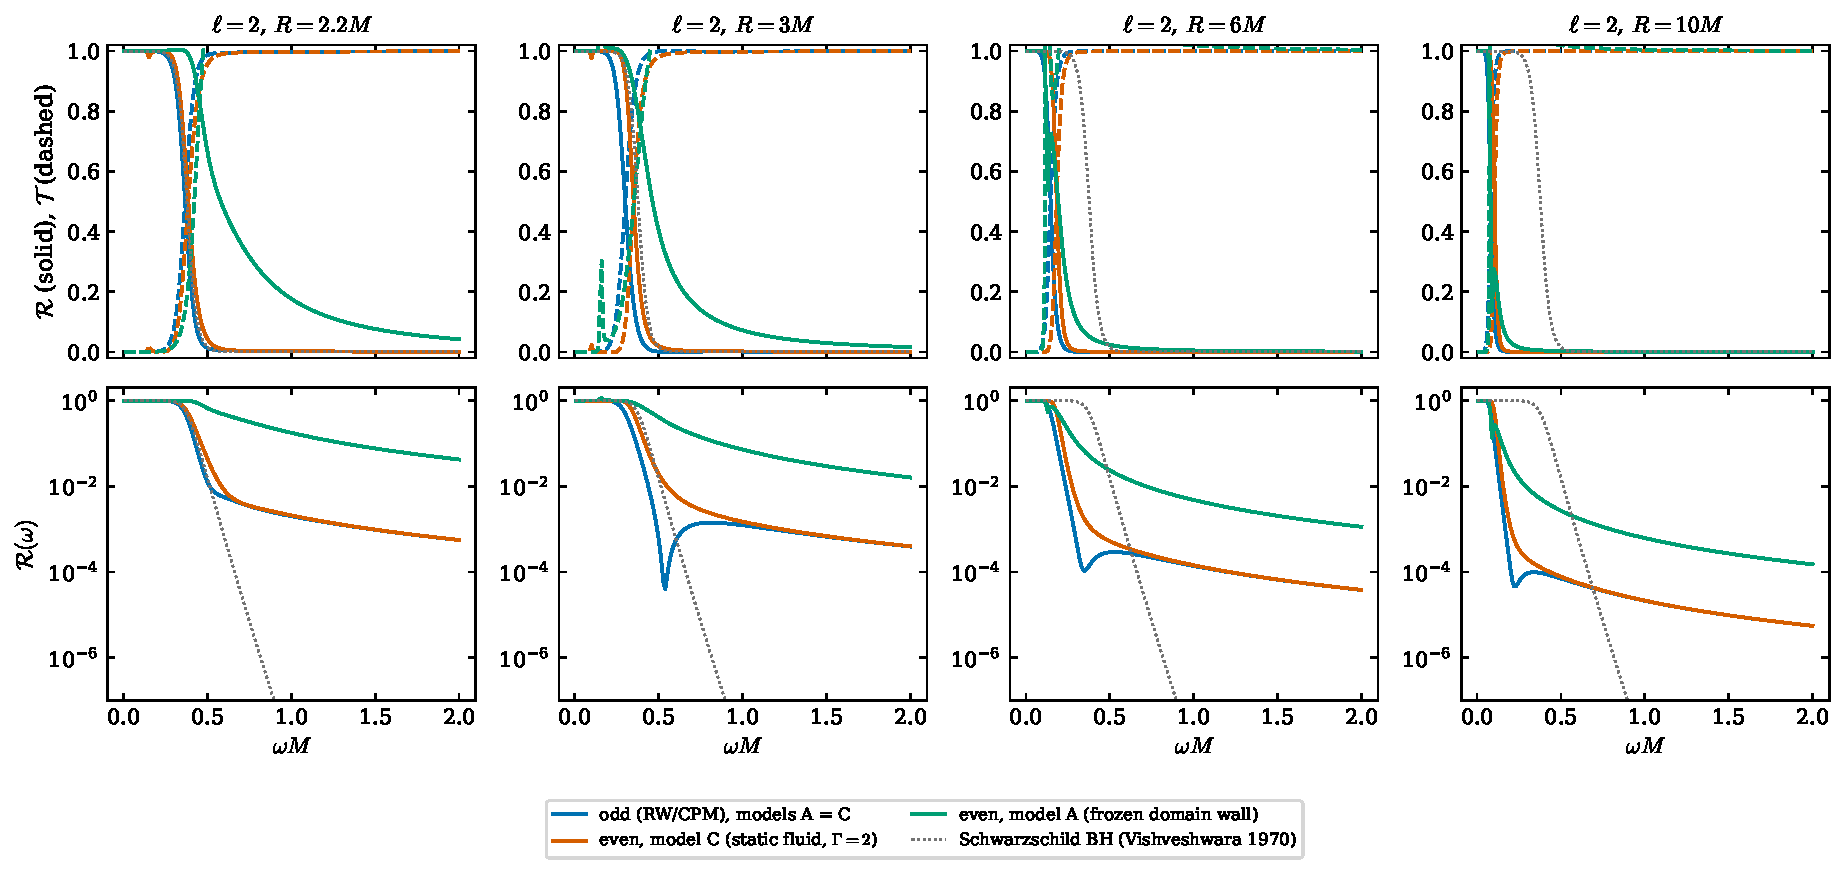
\includegraphics[width=\textwidth]{fig02_RT_l2.pdf}
\caption{$\RR$ (solid) and $\TT$ (dashed; top) and $\RR$ on a log scale (bottom), $\ell=2$, $R/M=2.2,3,6,10$. Blue: odd
(any model). Orange: even, model C ($\Gamma=2$). Green: even, model A (first-round prescription; see
Sec.~\ref{sec:evenA}). Grey: Schwarzschild black hole.}\label{fig:RT2}
\vspace{3mm}
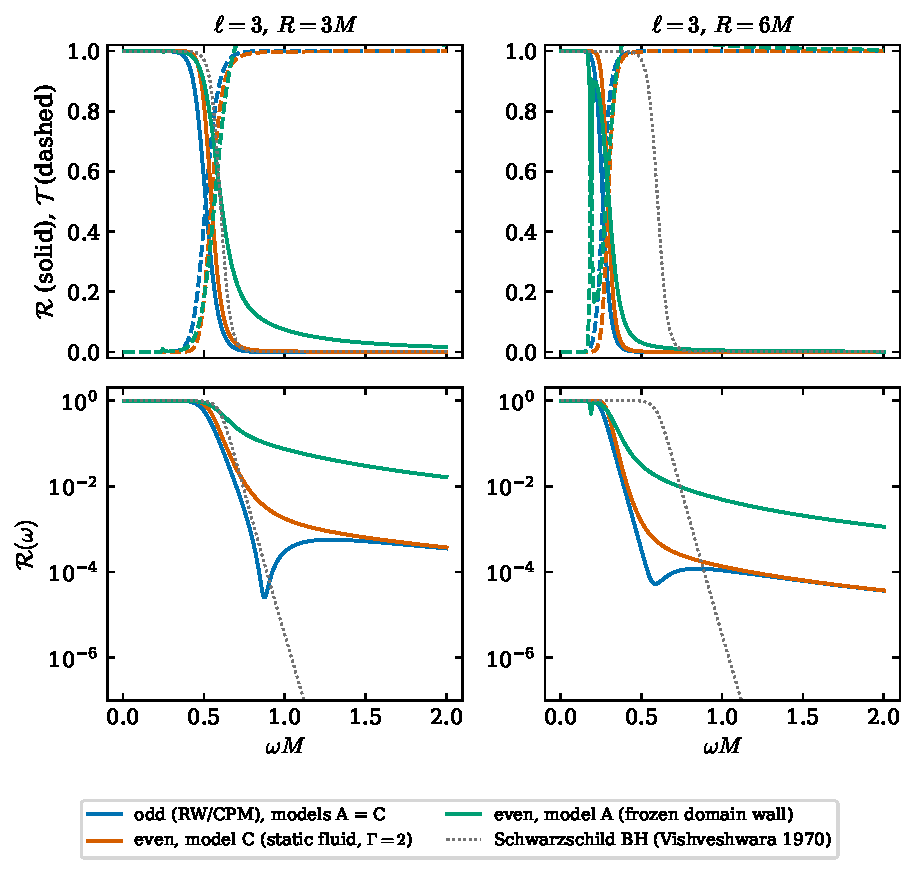
\includegraphics[width=0.49\textwidth]{fig03a_RT_l3.pdf}\hfill
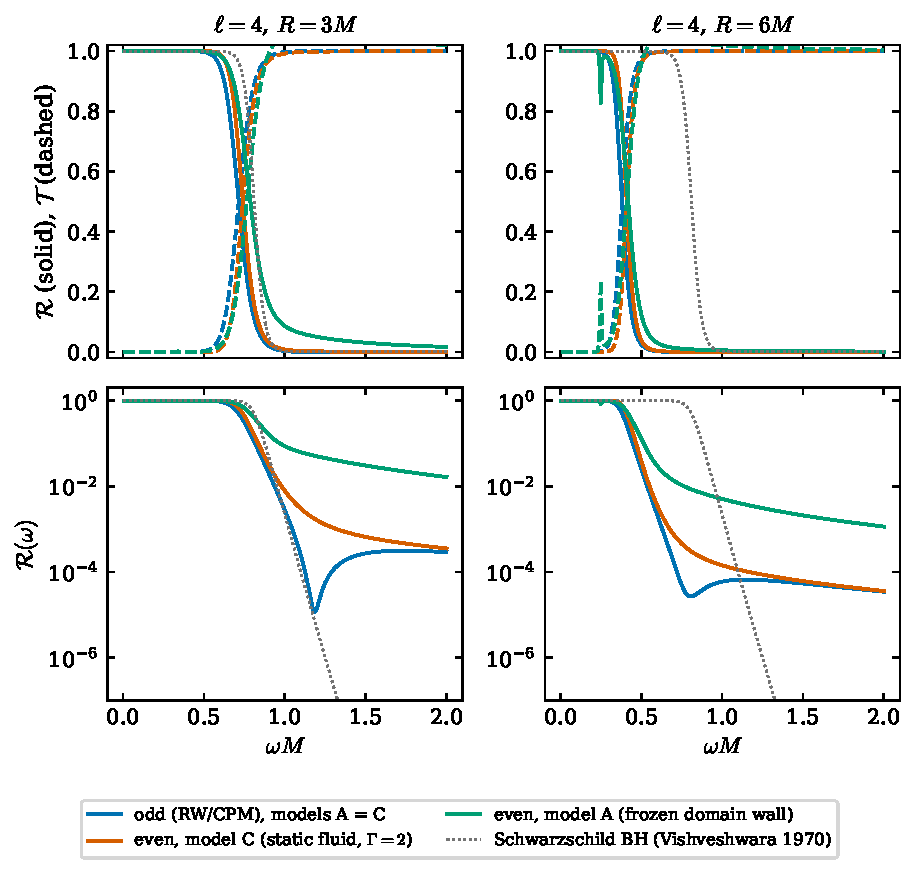
\includegraphics[width=0.49\textwidth]{fig03b_RT_l4.pdf}
\caption{As Fig.~\ref{fig:RT2} for $\ell=3$ (left) and $\ell=4$ (right), $R/M=3,6$.}\label{fig:RT34}
\end{figure}

\begin{figure}[t]\centering
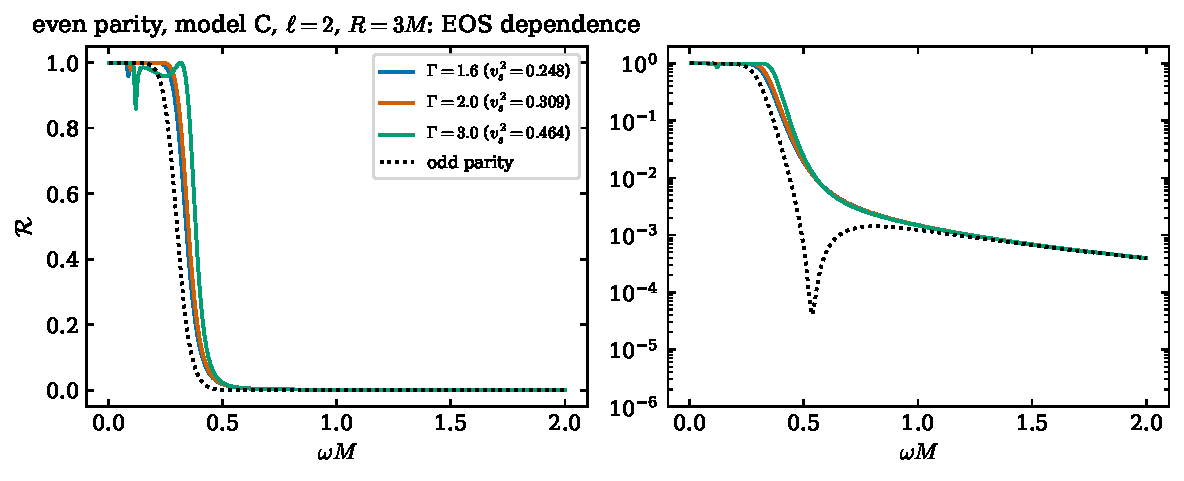
\includegraphics[width=0.85\textwidth]{fig04_eos_dependence.pdf}
\caption{Dependence of the even-parity reflectivity (model C, $\ell=2$, $R=3M$) on the adiabatic index.}\label{fig:eos}
\end{figure}

\begin{figure}[t]\centering
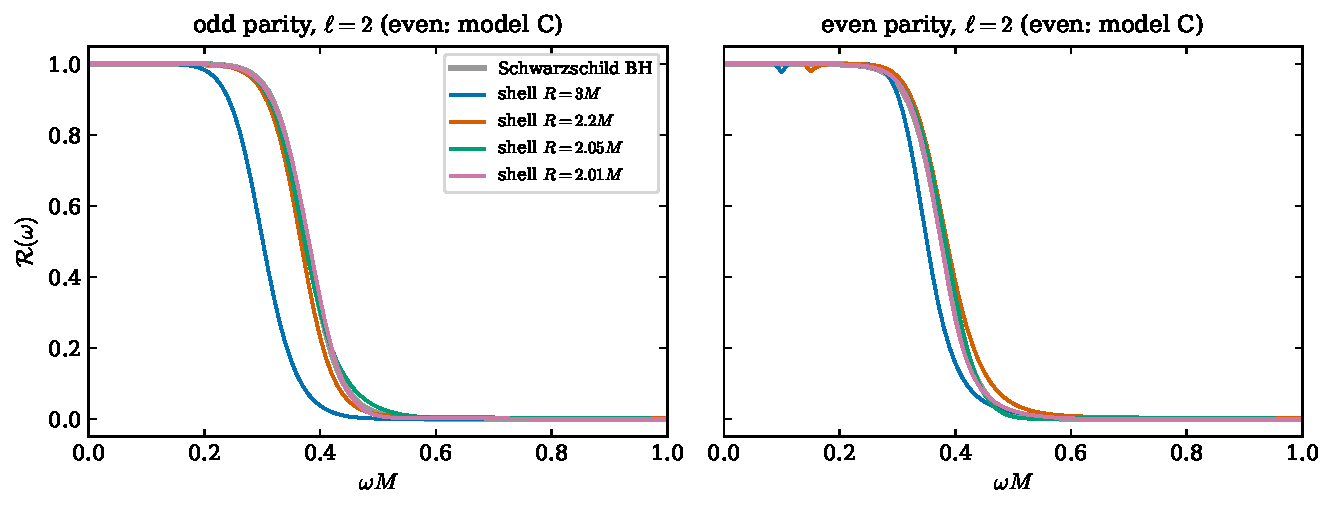
\includegraphics[width=0.8\textwidth]{fig09_schwarzschild_limit.pdf}\\
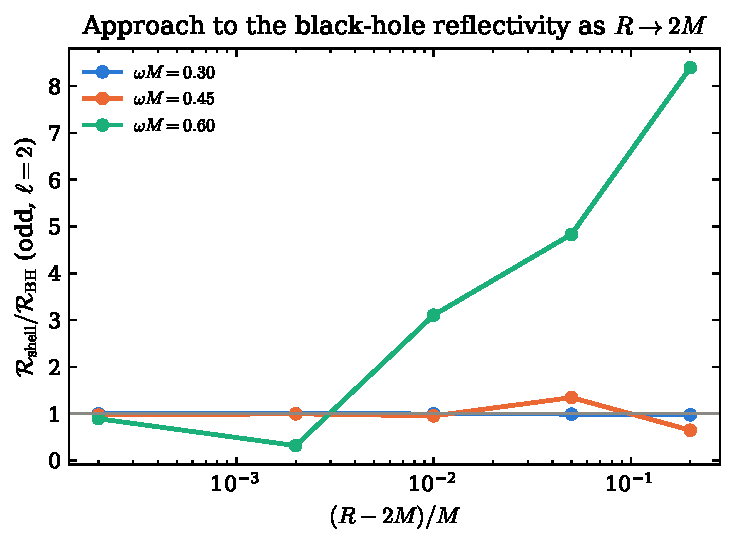
\includegraphics[width=0.5\textwidth]{r2_fig5_bh_limit.pdf}
\caption{Top: approach of the shell reflectivity to the black-hole value as $R\to2M$ (first round; see
Table~\ref{tab:bhlimit}). Bottom (second round): the approach is oscillatory and slow, with the shell contribution
scaling like $\Delta_{\rm odd}\propto(R-2M)^{1/2}$.}\label{fig:bhlimit}
\end{figure}
\begin{table}[h]\centering\small
\caption{Approach to the black-hole reflectivity ($\ell=2$; even: model C, 40 digits).}\label{tab:bhlimit}
\begin{tabular}{rrrrrrrr}\toprule
$\omega M$ & BH & odd $2.2M$ & odd $2.05M$ & odd $2.002M$ & even-C $2.2M$ & even-C $2.05M$ & even-C $2.01M$\\\midrule
0.20 & 0.99913 & 0.99886 & 0.99916 & 0.99907 & 0.99966 & 0.99921 & 0.99915\\
0.30 & 0.94521 & 0.92247 & 0.93661 & 0.94729 & 0.96577 & 0.95037 & 0.94996\\
0.37 & 0.56378 & 0.46896 & 0.52601 & 0.56105 & 0.62593 & 0.61107 & 0.54639\\
0.45 & 0.07559 & 0.04894 & 0.10167 & 0.07539 & 0.13163 & 0.07064 & 0.07361\\
0.60 & 0.00066 & 0.00554 & 0.00319 & 0.00021 & 0.00814 & 0.00166 & 0.00141\\
\bottomrule\end{tabular}

\end{table}

\subsection{Quasinormal modes}
The spectra are shown in the complex plane (Fig.~\ref{fig:qnmplane}) and as functions of $R/M$ (Fig.~\ref{fig:qnmR}).
\begin{itemize}
\item \emph{Wave modes} exist in both sectors, with $\omega\sim1/R$. For dilute shells PSP26 derived the Newtonian
law ${\rm Re}(\omega R)\simeq n\pi$ or $(n+\frac12)\pi$ and ${\rm Im}(\omega R)\simeq-\xi$, with
$\xi=\tfrac12\ln[2\ell(\ell+1)R/M]$ (their Eqs.~7.23--7.25). The interior cavity leaks through the weakly reflecting
shell, so the damping grows only logarithmically with $R/M$. Our wave modes coincide with PSP26's Figs.~3--4 to the
reading precision (Table~\ref{tab:psp}).
\item For compact shells ($R<3M$) a family of \emph{trapped} modes appears below the barrier top, damped only by
tunnelling. As $R\to2M$ they become exponentially long-lived and dense (Table~\ref{tab:trapped}). These are the modes
responsible for gravitational-wave ``echoes'' \cite{Cardoso2016PRL,Abedi2017}. None of them tends to a Schwarzschild QNM:
the black-hole spectrum is \emph{not} a limit of the shell spectrum, although the reflectivity is.
\item \emph{Matter modes} exist only in the even sector of model C (Sec.~\ref{sec:matter}).
\end{itemize}

\begin{figure}[t]\centering
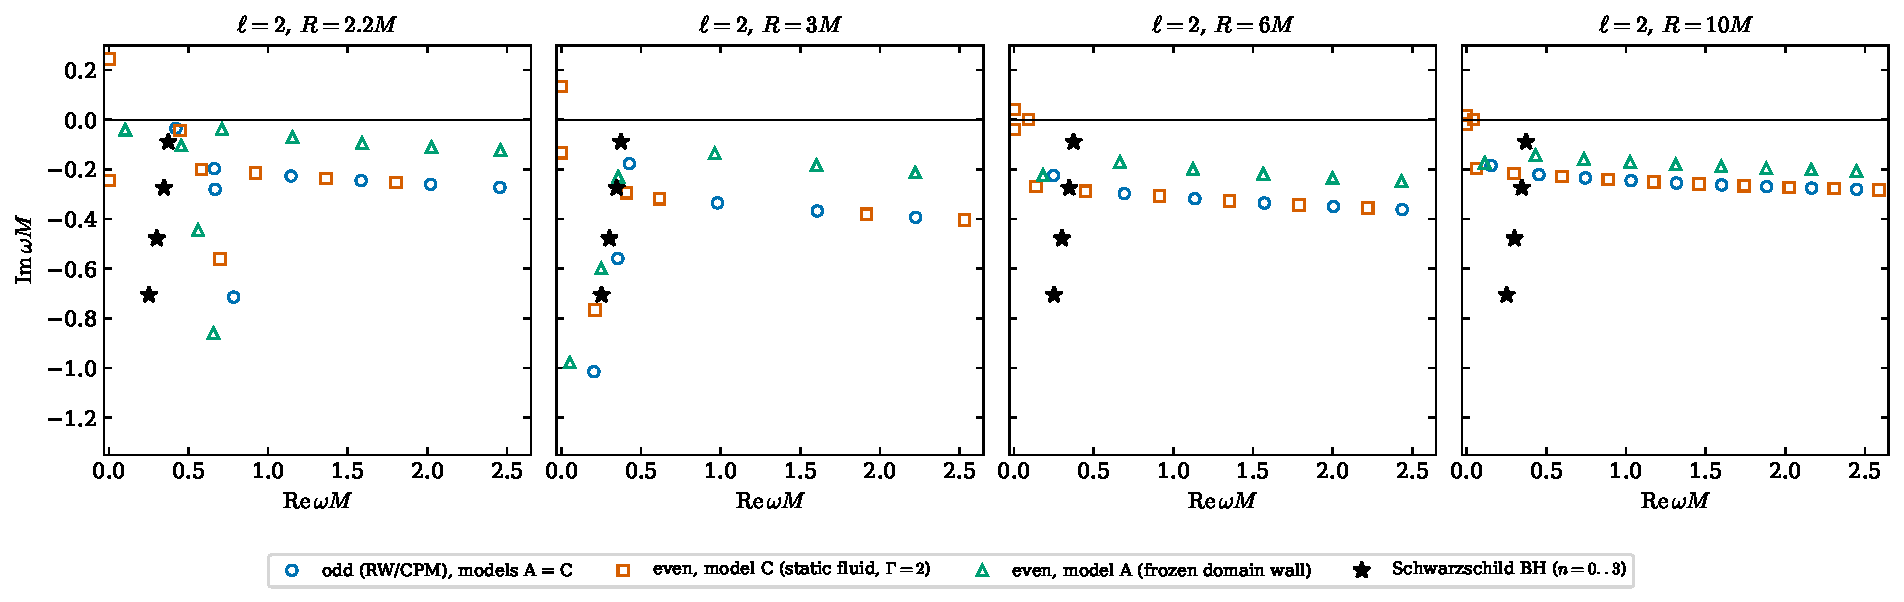
\includegraphics[width=\textwidth]{fig06_qnm_complex_plane.pdf}
\caption{QNMs for $\ell=2$: odd (circles), even model C (squares), even model A (triangles; first-round prescription)
and Schwarzschild (stars). The unstable matter mode lies on the positive imaginary axis.}\label{fig:qnmplane}
\end{figure}
\begin{figure}[t]\centering
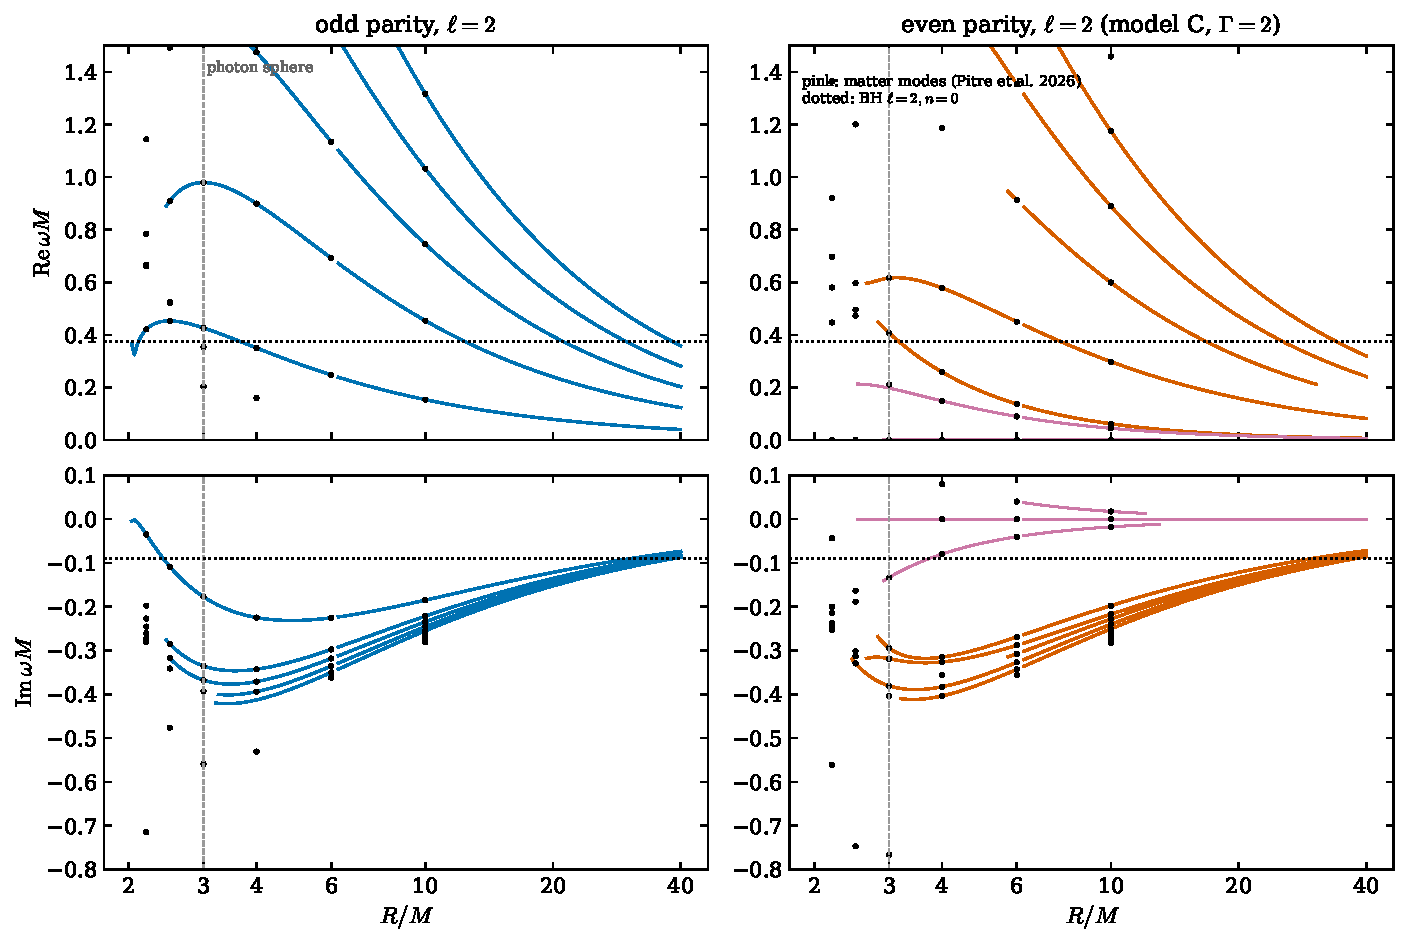
\includegraphics[width=\textwidth]{fig07_qnm_vs_compactness.pdf}
\caption{QNM frequencies vs $R/M$ for $\ell=2$ (continuation from $R=6M$; dots: independent scans).}\label{fig:qnmR}
\end{figure}

\begin{table}[h]\centering\small
\caption{Wave modes ($\ell=2$; even: model C, $\Gamma=2$) compared with PSP26 Figs.~3--4 (reading uncertainty
$\pm0.02$).}\label{tab:psp}
\begin{tabular}{lrrrrrr}\toprule
parity & $M/R$ & mode & ${\rm Re}(R\omega)$ & ${\rm Im}(R\omega)/\xi$ & PSP26 Re & PSP26 Im$/\xi$\\\midrule
odd & 0.167 & 1 & 1.484 & -0.632 & 1.47 & -0.630 \\
odd & 0.167 & 2 & 4.151 & -0.835 & 4.10 & -0.840 \\
even & 0.250 & 1 & 1.033 & -0.651 & 1.05 & -0.655 \\
even & 0.100 & 1 & 0.615 & -0.825 & 0.62 & -0.825 \\
even & 0.100 & 2 & 2.978 & -0.907 & 2.95 & -0.910 \\
\bottomrule\end{tabular}

\end{table}
\begin{table}[h]\centering\scriptsize
\caption{Lowest wave modes, $\ell=2$, from the first-round catalogue. The stable matter pair is missing at
$R=2.2M$ and $3M$ (see the box in Sec.~\ref{sec:matter}).}\label{tab:qnm2}
\begin{tabular}{rlp{12cm}}\toprule
$R/M$ & sector & lowest wave modes $\omega M$ (ordered by ${\rm Re}\,\omega$; Methods 1 and 2 agree to $<10^{-4}$)\\\midrule
2.2 & odd & $0.42111-0.03502i$, $0.66196-0.19736i$, $0.66692-0.28043i$, $0.78377-0.71437i$ \\
2.2 & even-C & $0.44694-0.04385i$, $0.57996-0.19970i$, $0.69756-0.56050i$, $0.92055-0.21412i$; matter: $0.00000+0.24429i$, $0.00000-0.24429i$ \\
2.2 & even-A & $0.10284-0.04070i$, $0.45445-0.10428i$, $0.56024-0.44388i$, $0.65595-0.85878i$ \\
3 & odd & $0.20371-1.01489i$, $0.35352-0.55904i$, $0.42638-0.17728i$, $0.97955-0.33508i$ \\
3 & even-C & $0.21102-0.76599i$, $0.40766-0.29425i$, $0.61594-0.31862i$, $1.91546-0.38053i$; matter: $-0.00000+0.13321i$, $-0.00000-0.13326i$ \\
3 & even-A & $0.05288-0.97817i$, $0.24913-0.59916i$, $0.35675-0.22995i$, $0.96224-0.13441i$ \\
6 & odd & $0.24739-0.22534i$, $0.69189-0.29749i$, $1.13482-0.31819i$, $1.57166-0.33553i$ \\
6 & even-C & $0.13710-0.26885i$, $0.45011-0.28793i$, $0.91288-0.30736i$, $1.35361-0.32702i$; matter: $0.08942-0.00005i$, $-0.00000+0.04014i$, $-0.00000-0.04014i$ \\
6 & even-A & $0.18120-0.22393i$, $0.66401-0.17021i$, $1.12337-0.19838i$, $1.56453-0.21844i$ \\
10 & odd & $0.15342-0.18490i$, $0.45405-0.22153i$, $0.74518-0.23457i$, $1.03239-0.24567i$ \\
10 & even-C & $0.06152-0.19748i$, $0.29784-0.21714i$, $0.59930-0.22783i$, $0.88902-0.24022i$; matter: $0.04421-0.00001i$, $-0.00000+0.01762i$, $0.00000-0.01762i$ \\
10 & even-A & $0.11383-0.17403i$, $0.43293-0.14212i$, $0.73603-0.15791i$, $1.02659-0.17041i$ \\
\bottomrule\end{tabular}

\end{table}
\begin{table}[h]\centering\small
\caption{Trapped modes of ultracompact shells (odd, $\ell=2$): exact vs WKB.}\label{tab:trapped}
\begin{tabular}{rll}\toprule
$R/M$ & exact (M1) & WKB (Bohr--Sommerfeld + Gamow)\\\midrule
2.01 & $0.162603-9.711e-07\,i$ & $0.152432-5.081e-07\,i$ \\
2.01 & $0.248683-5.284e-05\,i$ & $0.246194-3.249e-05\,i$ \\
2.01 & $0.326133-8.798e-04\,i$ & $0.328792-7.287e-04\,i$ \\
2.02 & $0.216610-1.809e-05\,i$ & $0.205905-8.922e-06\,i$ \\
2.02 & $0.322125-1.072e-03\,i$ & $0.324183-8.289e-04\,i$ \\
2.05 & $0.302815-8.384e-04\,i$ & $0.296095-4.811e-04\,i$ \\
2.10 & $0.367989-8.195e-03\,i$ & $0.370495-7.304e-03\,i$ \\
\bottomrule\end{tabular}

\end{table}

\subsection{Matter modes and the instability of the static shell}\label{sec:matter}
PSP26 found four even-parity matter modes per $\ell$: a purely imaginary unstable mode, its damped mirror, and a pair
$\pm{\rm Re}\,\omega+i\,{\rm Im}\,\omega$ with small negative imaginary part. They concluded that the shell is
dynamically unstable on all angular scales. Their method is different from ours. They use retarded-time slicing, an
RW-type master function in both sectors, and Chebyshev collocation or Mano--Suzuki--Takasugi (MST) type expansions.
Reproducing their results is therefore an independent test of our even junction (Table~\ref{tab:pitre},
Fig.~\ref{fig:pitre}). At $M/R=0.2$, $\Gamma=2$, $\ell=2$ we find $\omega(R^3/M)^{1/2}=0.60771i$ for the unstable mode
and $1.26707-0.00110i$ for the stable pair, as in PSP26 Figs.~1--2. As $M/R\to0$ the values approach the
post-Newtonian limits $0.51470i$ and $1.50496$ of PSP26 Eq.~(7.8), with $O(M/R)$ differences. The static model C is
therefore linearly unstable, with growth time $\simeq1.6(R^3/M)^{1/2}$.

\begin{table}[h]\centering\small
\caption{Even-parity matter modes, model C, $\ell=2$, $\Gamma=2$ ($|\Delta_{12}|$: M1--M2 difference).}\label{tab:pitre}
\begin{tabular}{rllll}\toprule
$M/R$ & unstable: $\omega(R^3/M)^{1/2}$ & $|\Delta_{12}|$ & stable pair: $\omega(R^3/M)^{1/2}$ & $|\Delta_{12}|$\\\midrule
0.30 & $0.668693\,i$ & 1.6e-12 & $1.095903-1.70e-03\,i$ & 1.8e-12 \\
0.25 & $0.636634\,i$ & 7.1e-12 & $1.188088-1.51e-03\,i$ & 9.2e-13 \\
0.20 & $0.607709\,i$ & 1.6e-11 & $1.267067-1.10e-03\,i$ & 3.9e-13 \\
0.15 & $0.581398\,i$ & 2.3e-11 & $1.336362-6.47e-04\,i$ & 5.1e-13 \\
0.10 & $0.557313\,i$ & 3.3e-11 & $1.398197-2.78e-04\,i$ & 6.1e-13 \\
0.05 & $0.535158\,i$ & 4.6e-11 & $1.454057-5.79e-05\,i$ & 7.4e-13 \\
0.02 & $0.522690\,i$ & 4.6e-11 & $1.485144-6.52e-06\,i$ & 8.3e-13 \\
0.01 & $0.518662\,i$ & 6.1e-11 & $1.495140-1.20e-06\,i$ & 0.0e+00 \\
$\to0$ (PN, PSP26 Eq.~7.8) & $0.514695\,i$ & & $1.504962$ & \\
\bottomrule\end{tabular}

\end{table}

\begin{figure}[t]\centering
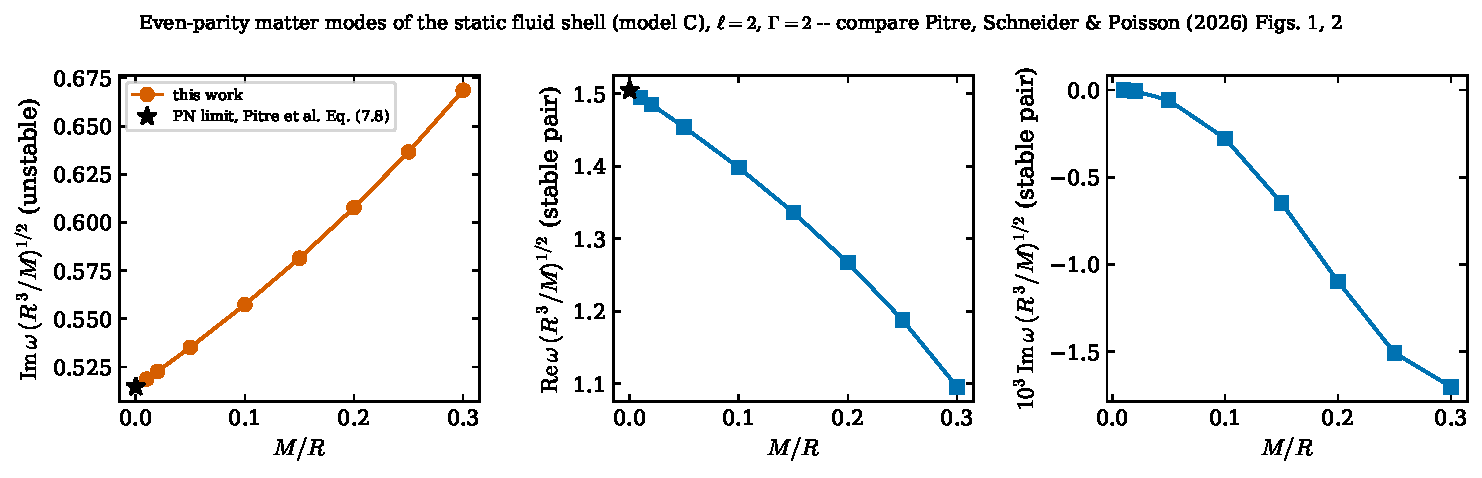
\includegraphics[width=\textwidth]{fig10_matter_modes_pitre.pdf}
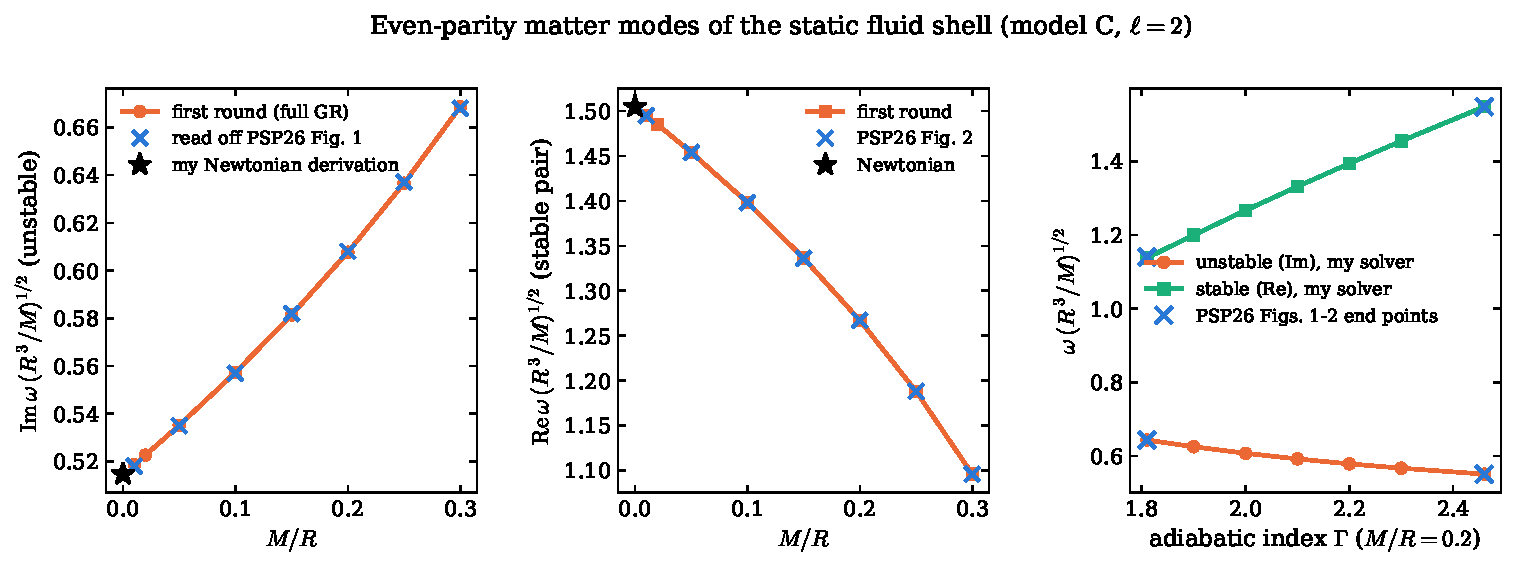
\includegraphics[width=\textwidth]{r2_fig2_matter_modes.pdf}
\caption{Top: matter modes vs compactness with the post-Newtonian limits (first round). Bottom (second round):
comparison with values read off PSP26, our Newtonian limit, and the $\Gamma$ dependence at $M/R=0.2$.}\label{fig:pitre}
\end{figure}

\begin{verifbox}
\textbf{Newtonian check.} The second round derived the non-radial oscillations of a Newtonian self-gravitating fluid
shell from scratch (App.~\ref{app:newton}) and recovered PSP26's Eq.~(7.8) identically, for all $\ell$ and $\Gamma$.
This also exposed a misprint in PSP26's quartic (7.6); its closed-form solution (7.8), used here, is correct. The
$\Gamma$ dependence (PSP26 Figs.~1--2, right panels) is reproduced as well. \textbf{Catalogue.} The first-round
catalogue misses the stable matter pair at $R=2.2,2.5,3M$ ($\ell=2$), e.g.\ $0.197121-0.000310i$ at $3M$, and the
unstable $\ell=4$ mode at $R=2.2M$ ($0.43726i$). These omissions do not change the conclusion: an unstable mode exists
for every $\ell$ and $R$ examined.
\end{verifbox}

%===============================================================================================
\section{Discussion}\label{sec:disc}
\paragraph{The shell model.} Neither a pure domain wall nor a dust shell has a static configuration; a static
shell needs positive surface pressure, $p/\sigma=(1-\sq)/4\sq$. Even that shell is dynamically unstable (PSP26,
confirmed). The ``collapse problem'' of the prior notes is thus generic, but its time scales differ. The fluid shell's
instability grows on $\sim1.6(R^3/M)^{1/2}$, which is long compared with the wave periods, so frequency-domain
scattering off model C is a meaningful adiabatic idealization for $\omega(R^3/M)^{1/2}\gg1$. The domain wall
collapses on $\sim R/\sqrt2$, comparable to the wave periods, and its frozen even-parity problem is not a controlled
approximation (Sec.~\ref{sec:evenA}).

\paragraph{Junction conditions.} In the odd sector, $[\Psi]=0$ and $[\partial_x\Psi]=\Delta_{\rm odd}\Psi$ hold with
$\Delta_{\rm odd}=\sq(1-\sq)/R$, independent of $\omega$ and of the equation of state. The $[K]^{(0)}$ term that worried
the prior notes cancels against $\delta S_{\tau A}$. The even sector gives a frequency-dependent $2\times2$ matrix,
because the shell's radial displacement differs between the two RW gauges and its compressional dynamics enter
through $v_s^2$.

\paragraph{Relation to previous work.} The odd junction agrees with PSP26 and with Pani et al.; the even junction
reproduces PSP26's matter and wave modes. Pani et al.'s gravastar has $\Sigma=0$ and a de Sitter interior, so only the
structure of the matching conditions can be compared; PSP26 argue that unstable modes should also exist in that
model. The new elements are:
\begin{itemize}
\item the reflection and transmission coefficients with their low-frequency, high-frequency and black-hole limits;
\item the explicit $\delta$-function form of the odd junction (and its thick-shell derivation);
\item a critical assessment of the frozen domain-wall model;
\item two independent numerical methods, and an independent third code in the verification round.
\end{itemize}

\paragraph{Limitations.} Model C is restricted to $R\ge25M/12$ by the energy and causality conditions. No
time-domain evolution of the unstable shell was attempted. The open-interior definition of $\RR$ and $\TT$ is a
convention adapted to the question ``how much of an incident wave is sent back by the barrier and the shell''; for the
closed physical system $|S|=1$.

\section{Conclusions}
A spherical thin shell with a flat interior is the simplest horizonless compact object, and its perturbation theory
can be carried out in closed form up to a $2\times2$ matching problem. The odd parity reduces to a $\delta$-potential,
the even parity to a transfer matrix that conserves flux exactly for the static fluid shell. Scattering interpolates
between perfect reflection at low frequency, the Schwarzschild reflectivity for $R\to2M$, and transparency at high
frequency. The QNM spectrum contains wave, trapped and matter modes, and the growing matter mode shows that the only
static member of the family is unstable. All of this was reproduced and cross-checked independently. The one
exception is the even sector of the frozen domain wall, which the frozen approximation does not determine.

%===============================================================================================
\appendix
\section{Newtonian oscillations of a self-gravitating fluid shell}\label{app:newton}
Consider a shell of radius $R$, surface density $\sigma$, two-dimensional pressure $p$ and mass $M=4\pi R^2\sigma$
($G=1$). The gravitational field acting on the shell is the average of the interior (zero) and exterior ($-M/R^2$)
fields. The normal force of a 2D fluid with pressure $p$ on a surface of mean curvature $2H$ is $2Hp$, outward.
Equilibrium therefore requires $2p/R=\sigma M/2R^2$, i.e.\ $p=\sigma M/4R$, the Newtonian limit of $\kappa$ in
Eq.~\eqref{eq:kappa}. Let the Lagrangian displacement be $\xi_rY\hat r+\xi_h\nabla_{S^2}Y$, with time dependence
$e^{-i\omega t}$, and define $x=\xi_r/R$ and $y=\xi_h/R$. Then:
\begin{itemize}
\item continuity: $\Delta\sigma/\sigma=-(2x-\lambda y)$, and $\Delta p=\Gamma p\,\Delta\sigma/\sigma$;
\item self-gravity: the displaced sheet acts on the exterior like a surface density $\sigma(\lambda y+\ell x)Y$ and on
the interior like $\sigma(\lambda y-(\ell+1)x)Y$ (the radial displacement shifts the multipole moments);
\item mean curvature: $2H=2/R-(2-\lambda)xY/R$.
\end{itemize}
With $\varsigma^2=\omega^2R^3/M$, the radial and tangential equations of motion become
\begin{align}
\varsigma^2x&=-x+\frac{\lambda(y+2x)}{2(2\ell+1)}+\frac\Gamma2(2x-\lambda y)+\frac{(2-\lambda)x}{4}-\frac{2x-\lambda y}{2},\\
\varsigma^2y&=-\frac\Gamma4(2x-\lambda y)-\frac{\lambda y-(\ell+1)x}{2\ell+1}.
\end{align}
The trace and determinant of this $2\times2$ problem are
\begin{equation}
\varsigma_+^2+\varsigma_-^2=\frac{(\ell^2+\ell+4)\Gamma-(\ell^2+\ell+6)}{4},\qquad
\varsigma_+^2\varsigma_-^2=-\frac{(\ell-1)\ell(\ell+1)[(\ell+2)(2\ell-3)\Gamma-4(\ell-2)]}{16(2\ell+1)} .
\end{equation}
The roots coincide identically with PSP26's Eq.~(7.8). Because the product is negative for $\Gamma>4(\ell-2)/[(\ell+2)(2\ell-3)]$,
one $\varsigma^2$ is negative, i.e.\ there is a purely imaginary growing mode: the Newtonian origin of the instability.
For $\ell=2$ and $\Gamma=2$ the roots are $\varsigma=1.504962$ and $0.514695\,i$. PSP26's Eq.~(7.6) prints the constant term as
$-(\ell-1)\ell(\ell+1)(\ell+2)[(2\ell-3)\Gamma-4]/[16(2\ell+1)]$. That form disagrees with (7.8) and with their own
Newtonian Eq.~(10.62), and for $\ell=2$ it would predict stability.

\section{Axial perturbations of an anisotropic fluid and the thin-shell limit}\label{app:axial}
For $\dd s^2=-e^{2\Phi}\dd t^2+e^{2\Lambda}\dd r^2+r^2\dd\Omega^2$, with $e^{-2\Lambda}=1-2m/r$ and
$T_{\mu\nu}=(\rho+p_t)u_\mu u_\nu+p_tg_{\mu\nu}+(p_r-p_t)s_\mu s_\nu$, consider an axial perturbation $h_0,h_1$ (RW
gauge) and $\delta u_\phi$. The $\theta\phi$ Einstein equation gives $h_0$ in terms of $h_1,h_1'$. The $r\phi$
equation then becomes, for $X=e^{\Phi-\Lambda}h_1/r$ and $\dd r_*=e^{\Lambda-\Phi}\dd r$,
\begin{equation}
X_{,r_*r_*}+\big\{\omega^2-e^{2\Phi}[\ell(\ell+1)/r^2-6m/r^3+4\pi(\rho-p_r)]\big\}X=0,
\end{equation}
once $m'=4\pi r^2\rho$, $\Phi'=(m+4\pi r^3p_r)/r(r-2m)$ and the anisotropic TOV equation
$p_r'=-(\rho+p_r)\Phi'+2(p_t-p_r)/r$ are used. For $p_r=0$ the TOV equation gives $p_t=\rho r\Phi'/2$. Integrating
across a layer whose thickness tends to zero, one finds $\int\rho\,\dd\ell_{\rm p}=(1-\sq)/4\pi R=\sigma$ and
$\int p_t\,\dd\ell_{\rm p}=(1-\sq)^2/16\pi R\sq=p$, exactly the model-C background. The only singular term of the
potential is $4\pi\rho e^{2\Phi}\to\Delta_{\rm odd}\delta(x-x_R)$ with $\Delta_{\rm odd}=4\pi\sigma\sq$. Since
$X\propto\Psi_{\rm CPM}$ on both sides, this is the junction \eqref{eq:oddfinal}.

\section{Code map and reproducibility}
\begin{tabular}{p{6.4cm}p{8.6cm}}
\toprule
\texttt{First round/code/main.py} & driver: \texttt{validate, scatter, qnm, tracks, csv, figures}\\
\texttt{symbolic/vacuum\_relations.py} & Einstein-tensor linearization; Eqs.~\eqref{eq:oddrecon}, \eqref{eq:Krec}--\eqref{eq:Hrec}\\
\texttt{symbolic/derive\_junction.py} & junction conditions; exports $\mathsf A$, $\mathsf B$\\
\texttt{symbolic/exterior\_series.py} & continued-fraction ODE; Chandrasekhar map\\
\texttt{shellgw/*.py} & background, interior, exterior, junction, scattering, QNM, black hole, WKB\\
\texttt{Second round/checks/*.py} & independent verification codes (companion report)\\\bottomrule
\end{tabular}

\medskip\noindent Re-running the first round reproduces \texttt{validation.json} bit for bit, all tables and all
figures (pixel-identical) and the symbolic junction matrices.

%===============================================================================================
\begin{thebibliography}{99}\small
\bibitem{RW57} T.~Regge and J.~A.~Wheeler, Stability of a Schwarzschild singularity, Phys.\ Rev.\ \textbf{108}, 1063 (1957).
\bibitem{Zerilli70} F.~J.~Zerilli, Effective potential for even-parity Regge--Wheeler gravitational perturbation equations, Phys.\ Rev.\ Lett.\ \textbf{24}, 737 (1970).
\bibitem{Vishveshwara70} C.~V.~Vishveshwara, Scattering of gravitational radiation by a Schwarzschild black-hole, Nature \textbf{227}, 936 (1970).
\bibitem{MP05} K.~Martel and E.~Poisson, Gravitational perturbations of the Schwarzschild spacetime: a practical covariant and gauge-invariant formalism, Phys.\ Rev.\ D \textbf{71}, 104003 (2005); K.~Martel, PhD thesis, University of Guelph (2004).
\bibitem{IS84} J.~Ipser and P.~Sikivie, Gravitationally repulsive domain wall, Phys.\ Rev.\ D \textbf{30}, 712 (1984).
\bibitem{Poisson04} E.~Poisson, \emph{A Relativist's Toolkit} (Cambridge University Press, 2004), Ch.~3.
\bibitem{AS72} M.~Abramowitz and I.~A.~Stegun, \emph{Handbook of Mathematical Functions} (Dover, 1972), Sec.~10.3.
\bibitem{DLMF} NIST Digital Library of Mathematical Functions, Ch.~10, \url{https://dlmf.nist.gov/10}.
\bibitem{ondas} Prior note \emph{Regular wave solutions of the interior Regge--Wheeler and Zerilli equations inside a thin spherical shell} (\texttt{Starting point/interior\_ondas\_cascara.pdf}).
\bibitem{burbuja} Prior note \emph{Gravitational-wave scattering off a thin-shell vacuum bubble, Part I} (\texttt{Starting point/burbuja\_matching\_israel.pdf}).
\bibitem{Pani09} P.~Pani, E.~Berti, V.~Cardoso, Y.~Chen and R.~Norte, Gravitational wave signatures of the absence of an event horizon. I. Nonradial oscillations of a thin-shell gravastar, Phys.\ Rev.\ D \textbf{80}, 124047 (2009), arXiv:0909.0287.
\bibitem{PSP26} T.~Pitre, B.~Schneider and E.~Poisson, Self-gravitating thin shells are dynamically unstable on all angular scales, Phys.\ Rev.\ D \textbf{113}, 124055 (2026), arXiv:2604.05980.
\bibitem{Boyanov25} V.~Boyanov, V.~Cardoso, K.~D.~Kokkotas and J.~Redondo-Yuste, Dynamical response of viscous objects to gravitational waves, Phys.\ Rev.\ Lett.\ \textbf{135}, 151402 (2025), arXiv:2411.16861.
\bibitem{YBP23} H.~Yang, B.~Bonga and Z.~Pan, Dynamical instability of self-gravitating membranes, Phys.\ Rev.\ Lett.\ \textbf{130}, 011402 (2023).
\bibitem{Leaver85} E.~W.~Leaver, An analytic representation for the quasi-normal modes of Kerr black holes, Proc.\ R.\ Soc.\ Lond.\ A \textbf{402}, 285 (1985).
\bibitem{Leaver90} E.~W.~Leaver, Quasinormal modes of Reissner--Nordstr\"om black holes, Phys.\ Rev.\ D \textbf{41}, 2986 (1990).
\bibitem{LNS93} M.~Leins, H.-P.~Nollert and M.~H.~Soffel, Nonradial oscillations of neutron stars: a new branch of strongly damped normal modes, Phys.\ Rev.\ D \textbf{48}, 3467 (1993).
\bibitem{Gautschi67} W.~Gautschi, Computational aspects of three-term recurrence relations, SIAM Rev.\ \textbf{9}, 24 (1967).
\bibitem{BCS09} E.~Berti, V.~Cardoso and A.~O.~Starinets, Quasinormal modes of black holes and black branes, Class.\ Quantum Grav.\ \textbf{26}, 163001 (2009).
\bibitem{SW85} B.~F.~Schutz and C.~M.~Will, Black hole normal modes: a semianalytic approach, Astrophys.\ J.\ Lett.\ \textbf{291}, L33 (1985).
\bibitem{IW87} S.~Iyer and C.~M.~Will, Black-hole normal modes: a WKB approach. I, Phys.\ Rev.\ D \textbf{35}, 3621 (1987).
\bibitem{Iyer87} S.~Iyer, Black-hole normal modes: a WKB approach. II. Schwarzschild black holes, Phys.\ Rev.\ D \textbf{35}, 3632 (1987).
\bibitem{Konoplya03} R.~A.~Konoplya, Quasinormal behavior of the D-dimensional Schwarzschild black hole and higher order WKB approach, Phys.\ Rev.\ D \textbf{68}, 024018 (2003).
\bibitem{Hatsuda20} Y.~Hatsuda, Quasinormal modes of black holes and Borel summation, Phys.\ Rev.\ D \textbf{101}, 024008 (2020).
\bibitem{Killingbeck78} J.~Killingbeck, Perturbation theory without wavefunctions, Phys.\ Lett.\ A \textbf{65}, 87 (1978).
\bibitem{FernandezCastro87} F.~M.~Fern\'andez and E.~A.~Castro, \emph{Hypervirial Theorems}, Lecture Notes in Chemistry \textbf{43} (Springer, 1987).
\bibitem{BenderWu69} C.~M.~Bender and T.~T.~Wu, Anharmonic oscillator, Phys.\ Rev.\ \textbf{184}, 1231 (1969).
\bibitem{Langer37} R.~E.~Langer, On the connection formulas and the solutions of the wave equation, Phys.\ Rev.\ \textbf{51}, 669 (1937).
\bibitem{Chandrasekhar83} S.~Chandrasekhar, \emph{The Mathematical Theory of Black Holes} (Oxford University Press, 1983), Ch.~4.
\bibitem{ChandrasekharFerrari91} S.~Chandrasekhar and V.~Ferrari, On the non-radial oscillations of a star. III. A reconsideration of the axial modes, Proc.\ R.\ Soc.\ Lond.\ A \textbf{434}, 449 (1991).
\bibitem{ThorneCampolattaro67} K.~S.~Thorne and A.~Campolattaro, Non-radial pulsation of general-relativistic stellar models. I, Astrophys.\ J.\ \textbf{149}, 591 (1967).
\bibitem{Kojima92} Y.~Kojima, Equations governing the nonradial oscillations of a slowly rotating relativistic star, Phys.\ Rev.\ D \textbf{46}, 4289 (1992).
\bibitem{CPM78} C.~T.~Cunningham, R.~H.~Price and V.~Moncrief, Radiation from collapsing relativistic stars. I, Astrophys.\ J.\ \textbf{224}, 643 (1978).
\bibitem{Moncrief74} V.~Moncrief, Gravitational perturbations of spherically symmetric systems. I. The exterior problem, Ann.\ Phys.\ (N.Y.) \textbf{88}, 323 (1974).
\bibitem{Lanczos24} K.~Lanczos, Fl\"achenhafte Verteilung der Materie in der Einsteinschen Gravitationstheorie, Ann.\ Phys.\ (Leipzig) \textbf{74}, 518 (1924).
\bibitem{Israel66} W.~Israel, Singular hypersurfaces and thin shells in general relativity, Nuovo Cimento B \textbf{44}, 1 (1966).
\bibitem{MazurMottola04} P.~O.~Mazur and E.~Mottola, Gravitational vacuum condensate stars, Proc.\ Natl.\ Acad.\ Sci.\ \textbf{101}, 9545 (2004).
\bibitem{VisserWiltshire04} M.~Visser and D.~L.~Wiltshire, Stable gravastars -- an alternative to black holes?, Class.\ Quantum Grav.\ \textbf{21}, 1135 (2004).
\bibitem{ChirentiRezzolla07} C.~B.~M.~H.~Chirenti and L.~Rezzolla, How to tell a gravastar from a black hole, Class.\ Quantum Grav.\ \textbf{24}, 4191 (2007).
\bibitem{CardosoPani2019} V.~Cardoso and P.~Pani, Testing the nature of dark compact objects: a status report, Living Rev.\ Relativ.\ \textbf{22}, 4 (2019).
\bibitem{Cardoso2016PRL} V.~Cardoso, E.~Franzin and P.~Pani, Is the gravitational-wave ringdown a probe of the event horizon?, Phys.\ Rev.\ Lett.\ \textbf{116}, 171101 (2016).
\bibitem{Cardoso2016PRD} V.~Cardoso, S.~Hopper, C.~F.~B.~Macedo, C.~Palenzuela and P.~Pani, Gravitational-wave signatures of exotic compact objects and of quantum corrections at the horizon scale, Phys.\ Rev.\ D \textbf{94}, 084031 (2016).
\bibitem{Abedi2017} J.~Abedi, H.~Dykaar and N.~Afshordi, Echoes from the abyss: tentative evidence for Planck-scale structure at black hole horizons, Phys.\ Rev.\ D \textbf{96}, 082004 (2017).
\bibitem{KokkotasSchmidt99} K.~D.~Kokkotas and B.~G.~Schmidt, Quasi-normal modes of stars and black holes, Living Rev.\ Relativ.\ \textbf{2}, 2 (1999).
\bibitem{Nollert99} H.-P.~Nollert, Quasinormal modes: the characteristic `sound' of black holes and neutron stars, Class.\ Quantum Grav.\ \textbf{16}, R159 (1999).
\bibitem{KonoplyaZhidenko11} R.~A.~Konoplya and A.~Zhidenko, Quasinormal modes of black holes: from astrophysics to string theory, Rev.\ Mod.\ Phys.\ \textbf{83}, 793 (2011).
\bibitem{Hairer93} E.~Hairer, S.~P.~N{\o}rsett and G.~Wanner, \emph{Solving Ordinary Differential Equations I} (Springer, 1993).
\bibitem{SciPy20} P.~Virtanen \emph{et al.}, SciPy 1.0: fundamental algorithms for scientific computing in Python, Nat.\ Methods \textbf{17}, 261 (2020); A.~Meurer \emph{et al.}, SymPy: symbolic computing in Python, PeerJ Comput.\ Sci.\ \textbf{3}, e103 (2017); F.~Johansson \emph{et al.}, mpmath, \url{https://mpmath.org}.
\end{thebibliography}

\end{document}
